\documentclass[a4paper,10pt]{scrbook}
\usepackage[italian]{babel}
\usepackage[utf8x]{inputenc}
\usepackage{amsmath}
\usepackage{amsthm}
\usepackage{amssymb}
\usepackage{amscd}
\usepackage{graphicx}
\usepackage{float}
\usepackage{array}
\usepackage{rotating}
\usepackage{caption}
\usepackage{lscape}
\usepackage{fancybox}
\usepackage{hyperref}
\hypersetup{
    bookmarks=true,         % show bookmarks bar?
    unicode=false,          % non-Latin characters in Acrobat’s bookmarks
    pdftoolbar=true,        % show Acrobat’s toolbar?
    pdfmenubar=true,        % show Acrobat’s menu?
    pdffitwindow=false,     % window fit to page when opened
    pdfstartview={FitH},    % fits the width of the page to the window
    pdftitle={Sigurd  Cms},    % title
    pdfauthor={Matteo Mosangini},     % author
    pdfsubject={Gestione Cms scolastico},   % subject of the document
    pdfcreator={Matteo Mosangini},   % creator of the document
    pdfproducer={Matteo Mosangini}, % producer of the document
    pdfkeywords={cms ezpublish sigurd scuola alunni}, % list of keywords
    pdfnewwindow=true,      % links in new window
    colorlinks=false,       % false: boxed links; true: colored links
    linkcolor=red,          % color of internal links
    citecolor=green,        % color of links to bibliography
    filecolor=magenta,      % color of file links
    urlcolor=cyan           % color of external links
}


\renewcommand{\textfraction}{0.05}
\renewcommand{\topfraction}{0.95}
\renewcommand{\bottomfraction}{0.95}
\renewcommand{\floatpagefraction}{0.35}

\setcounter{totalnumber}{5}
\restylefloat{figure}
\newlength{\drop}


\newcommand{\titleBWF}{\begingroup% Beowulf
\drop = 0.1\textheight
\parindent=0pt
\vspace{\drop}
{\Huge\bfseries Cms Scolastico}\\[\baselineskip]
{\Large {\itshape Guida} {\scshape per l'utente}}\par
\vspace{5cm}
\begin{center}
\includegraphics[width=0.4\textwidth]{./immagini/logo/sigurd2.png}
\end{center}
\centering
{\Huge\bfseries S.I.G.U.R.D}\footnote{Sistema integrato gestione unificata risorse didattiche}

{\Large\itshape }
\vspace*{\drop}
\endgroup}


\begin{document}





\begin{titlepage}
 \titleBWF
\end{titlepage}

\tableofcontents
\chapter[Installazione]{Installazione e deployment}

\section{Installazione}
Per effettuare l'installazione creiamo una directory all'interno di \textsl{/var/www} entro cui copieremo il codice del nostro sito.

\begin{verbatim}
cd /var/www
mkdir <siteroot>
\end{verbatim}

ovviamente al posto di \textsl{siteroot} userete il nome da voi scelto. Dobbiamo ora decomprimere all'interno di questa directory i file sorgente di base del sito che si trovano all'interno del file compresso \textbf{sigurdbase.tar.bz2}.

\begin{verbatim}
cd <siteroot>
tar jxvf /tmp/sigurdbase.tar.bz2
\end{verbatim}

\subsection{Configurazione di Apache}

Dobbiamo ora configurare un Virtual host per Apache al fine di rendere accessibile il nostro sito al mondo esterno. Il file di configurazione base è:
\begin{verbatim}
NameVirtualHost 192.168.0.5:80
<VirtualHost 192.168.0.5:80>
ServerAdmin administrator@ilmiosito.it
ServerName www.ilmiosito.it
AcceptPathInfo On
DocumentRoot /var/www/<siteroot>
RewriteEngine On
RewriteCond %{HTTP_HOST} ^webdav\..*
RewriteRule ^(.*) /webdav.php [L]
Rewriterule ^/design/[^/]+/(stylesheets|images|javascript)/.* - [L]
AddOutputFilterByType DEFLATE text/html text/plain text/xml
ServerAlias webdav.ilmiosito.it
ServerAlias webadmin.ilmiosito.it
ServerAlias eng.ilmiosito.it
<Directory /var/www/<siteroot> >
Options Indexes FollowSymLinks MultiViews
AllowOverride All
Order allow,deny
allow from all
</Directory>
DirectoryIndex index.php
Rewriterule ^/var/storage/.* - [L]
RewriteRule ezjscore/call/ /index_ajax.php [L]
Rewriterule ^/var/[^/]+/storage/.* - [L]
RewriteRule ^/var/cache/texttoimage/.* - [L]
RewriteRule ^/var/[^/]+/cache/texttoimage/.* - [L]
Rewriterule ^/design/[^/]+/(stylesheets|images|javascript)/.* - [L]
Rewriterule ^/share/icons/.* - [L]
Rewriterule ^/extension/[^/]+/design/[^/]+/ \
	(lib|stylesheets|images|javascripts?)/.*  - [L]
Rewriterule  ^/packages/styles/.+/\ 
	(stylesheets|images|javascript)/[^/]+/.* - [L]
RewriteRule ^/packages/styles/.+/thumbnail/.* - [L]
RewriteRule ^/favicon\.ico - [L]
RewriteRule ^/robots\.txt - [L]
RewriteRule ^/var/[^/]+/cache/public/.* - [L]
RewriteRule .* /index.php
ErrorLog /var/log/apache2/ilmiositoerror.log LogLevel warn
CustomLog /var/log/apache2/ilmiositocustomlog.log combined
ServerSignature On
</VirtualHost>
\end{verbatim}








\chapter[Strutture]{Struttura dei contenuti}

\begin{sidewaysfigure}
 \centering
 \includegraphics[height=\textheight]{./immagini/strutture/organigramma_sito.png}
 % organigramma.pdf: 792x612 pixel, 72dpi, 27.94x21.59 cm, bb=
 \caption{Organigramma dei contenuti del sito}
 \label{fig:strutt_1}
\end{sidewaysfigure}
\begin{sidewaysfigure}
 \centering
 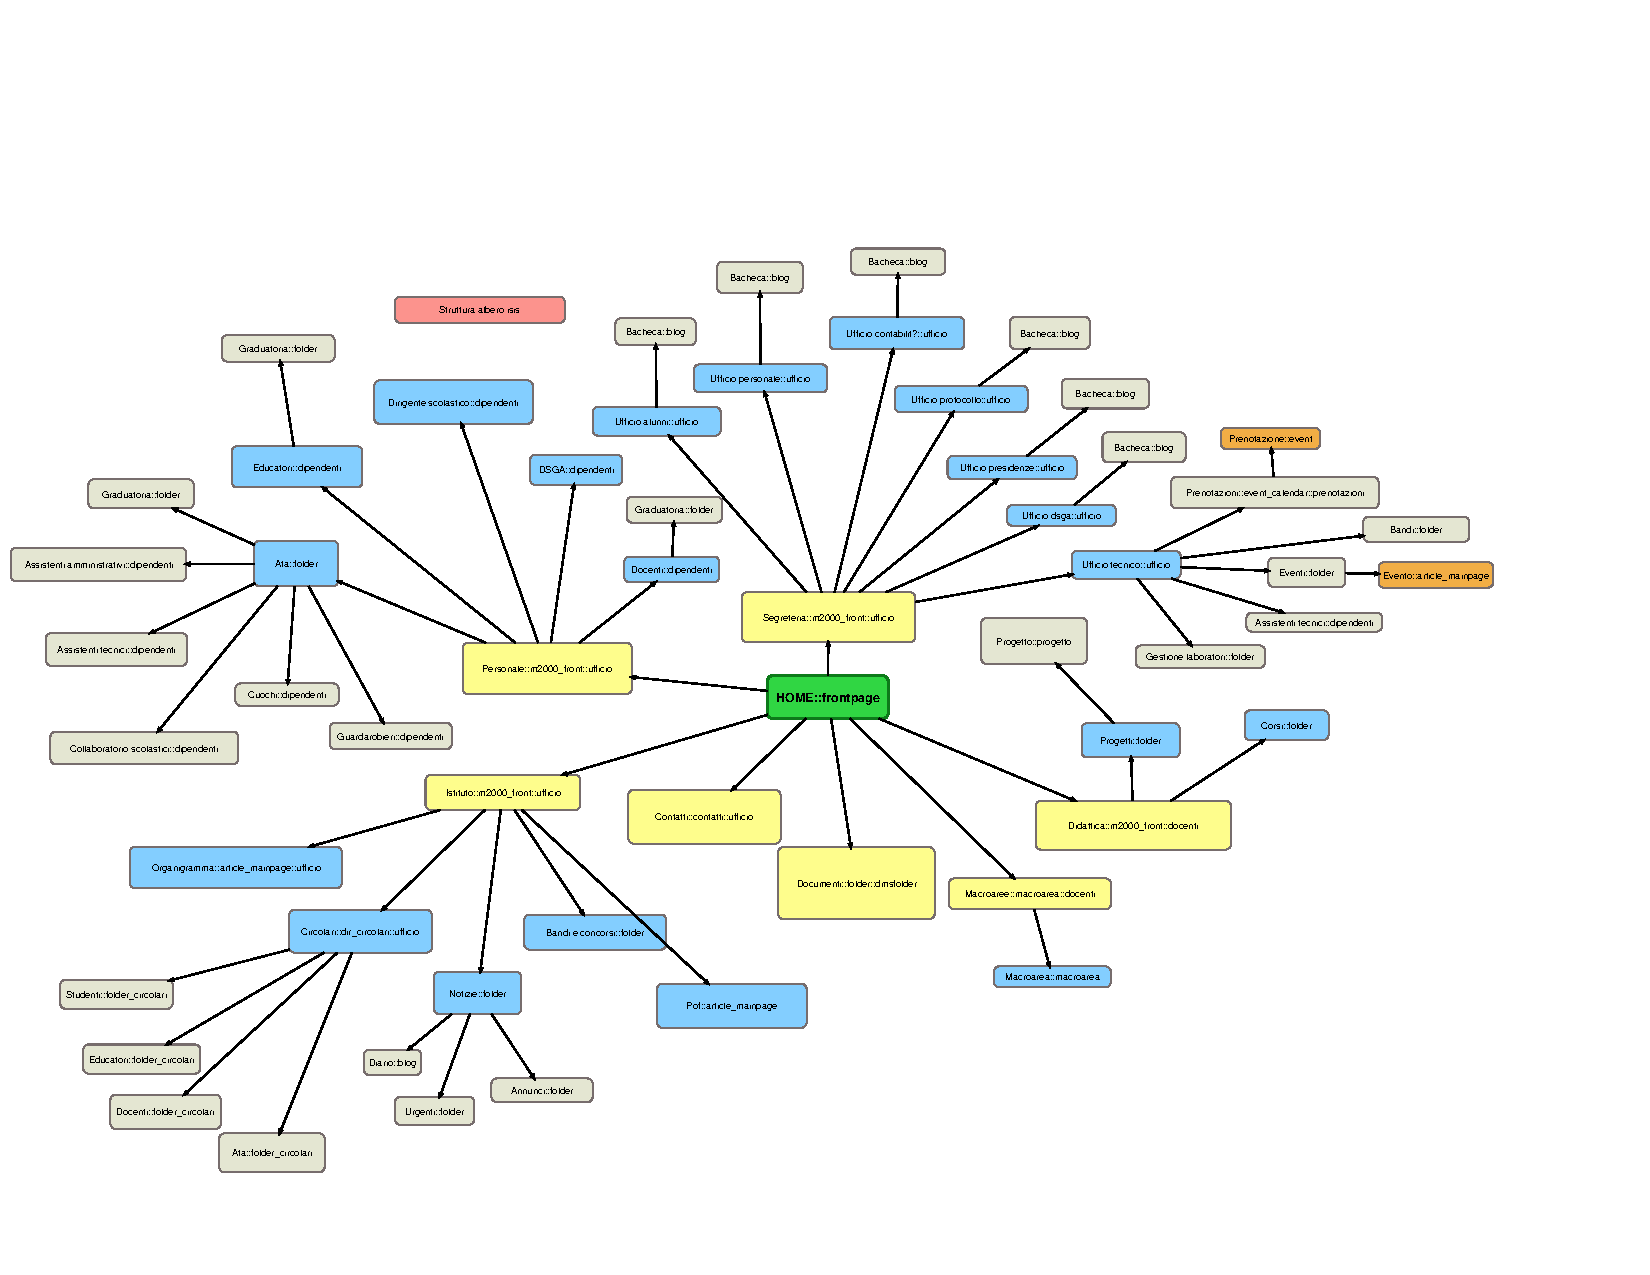
\includegraphics[height=\textheight]{./immagini/strutture/struttura_isis.pdf}
 % struttura_isis.pdf: 792x612 pixel, 72dpi, 27.94x21.59 cm, bb=
\caption{Struttura dei contenuti come implementata in EzPublish} 
\label{fig:strutt_2}
\end{sidewaysfigure}
\begin{sidewaysfigure}
 \flushleft
 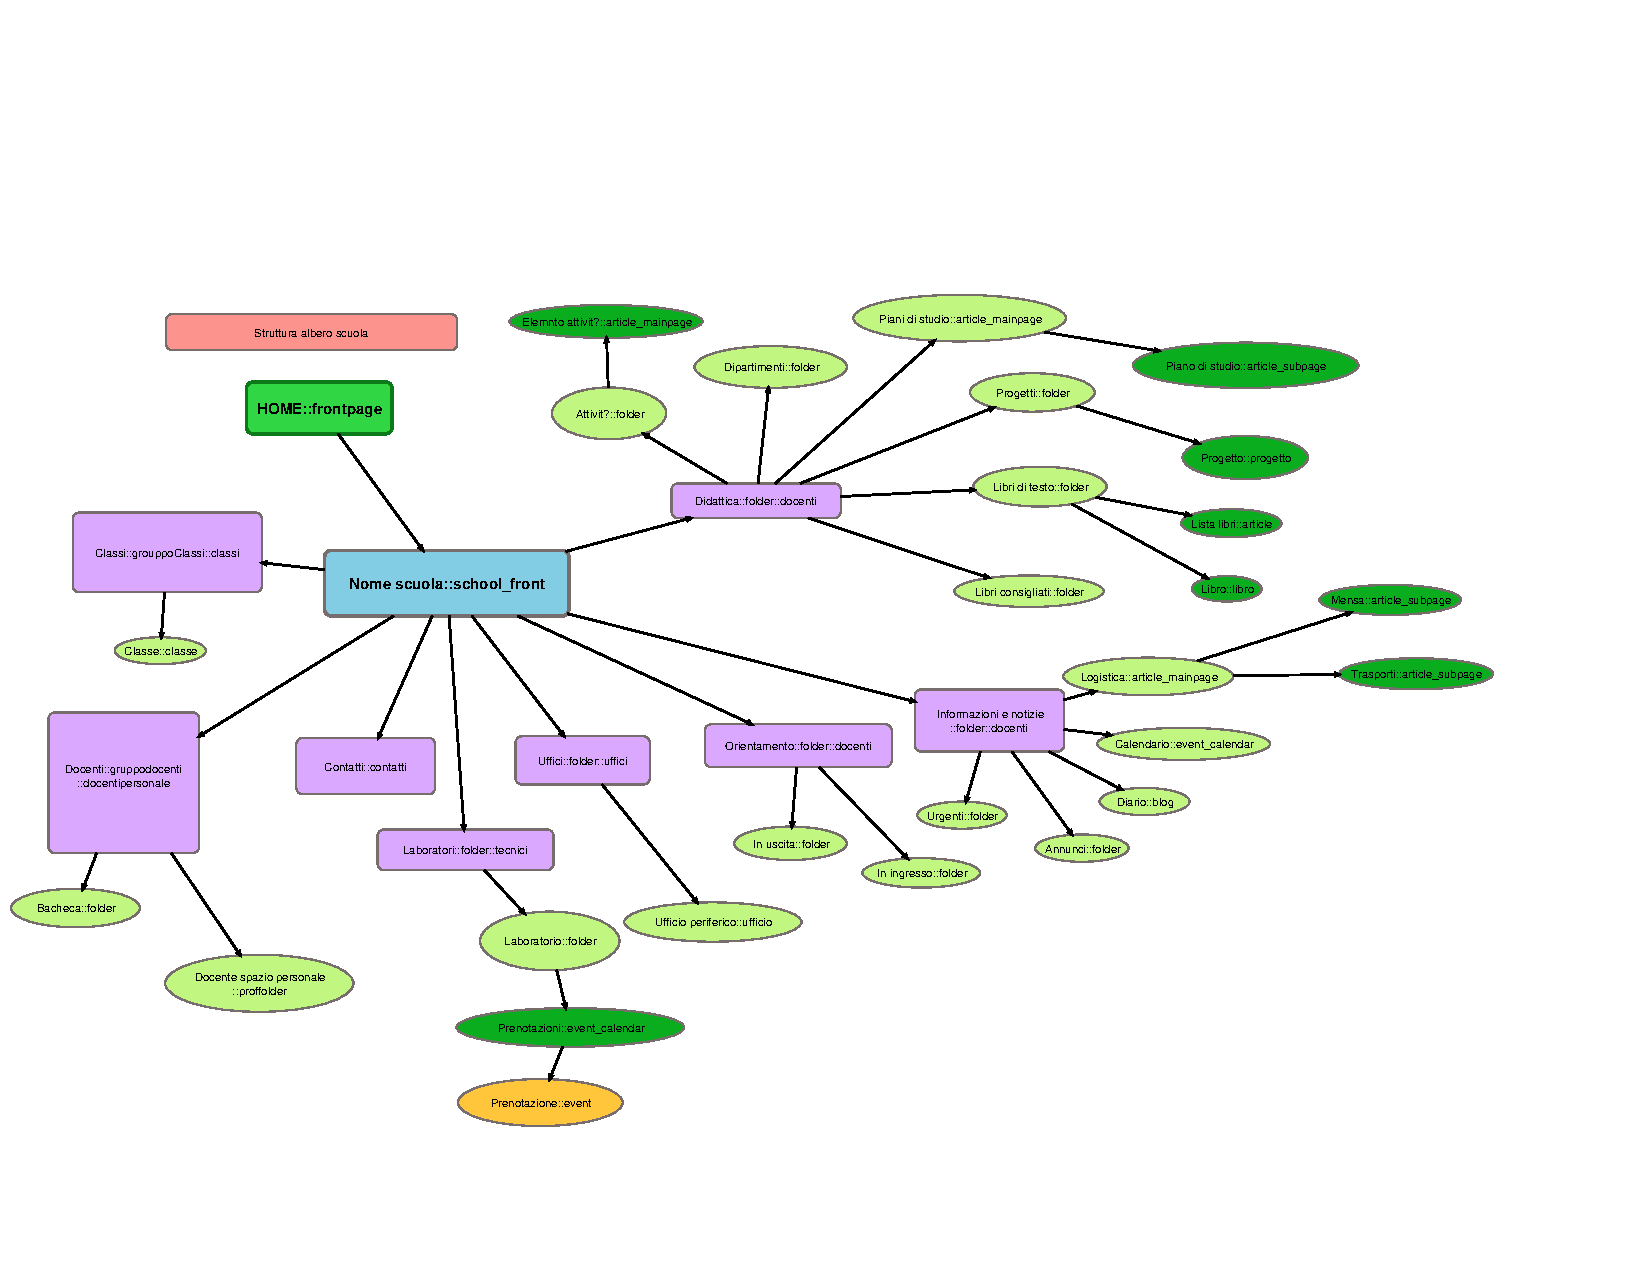
\includegraphics[height=\textheight]{./immagini/strutture/struttura_scuola.pdf}
 % struttura_scuola.pdf: 792x612 pixel, 72dpi, 27.94x21.59 cm, bb=0 0 792 612
\caption{Struttura dei contenuti di ogni singola scuola come implementata in EzPublish} 
\label{fig:strutt_scuola}
\end{sidewaysfigure}

\chapter[Registrazione]{La registrazione degli utenti}

Attualmente il sito prevede la presenza di quattro classi di utenti:

\begin{itemize}
 \item Genitori
\item Professori
\item Ata
\item Alunni
\end{itemize}


Dopo aver selezionato il collegamento \emph{Registrati} l'utente ha la possibilità di scegliere tra le classi prima illustrate quella più affine.

\begin{figure}[H]
 \centering
 \includegraphics[width=0.8\textwidth]{./immagini/registrazione/scelta_genere.png}
 % scelta_genere.png: 524x362 pixel, 72dpi, 18.49x12.77 cm, bb=
 \caption{Selezione del tipo di utente}
 \label{fig:reg_sel}
\end{figure}
Per ogni classe di utenti verrà presentata dal sistema una diversa form dedicata all'inserimento dei dati personali:
\begin{itemize}
 \item Genitori
\begin{itemize}
 \item Nome, Cognome, Dati account
\item Scuola frequentata dai figli
\item Figli frequentanti le varie scuole
\end{itemize}
\item Professori
\begin{itemize}
 \item Nome, Cognome, Dati account
\item Scuole di appartenenza
\item Classi di docenza
\item Sedi geografice di insegnamento
\end{itemize}
\item Ata
\begin{itemize}
 \item Nome, Cognome, Dati account
\item Scuole di appartenenza
\item Mansione
\end{itemize}
\item Alunni
\begin{itemize}
 \item Nome, Cognome, Dati account
\item Scuola frequentata
\end{itemize}
\end{itemize}


\section{Registrazione insegnante}

Durante la fase di registrazione l'insegnante è tenuto ad inserire:
\begin{description}
 \item[Nome e cognome] Il proprio nome e cognome con cui l'insegnante potrà essere individuato all'interno dell'istituto
\item[Account] Il sistema richiede il nome utente preferibilmente della forma \textbf{nome.cognome} e la password per accedere al sito. Si consiglia di utilizzare una password alfanumerica.
\item[Firma] Una frase da riportare nel proprio spazio utente
\item[Avatar] Una foto o un disegno rappresentanti l'utente
\item[Istituti] L'istituto o gli istituti in cui l'insegnante lavora
\item[Classi] Le classi di docenza del presente anno scolastico. Le scelte fatte durante il processo di registrazione circa le classi potranno essere modificate in qualsiasi momento
\item[Sede geografica] La sede o le sedi geografiche in cui l'insegnante lavora 
\end{description}

\begin{figure}[H]
 \centering
 \includegraphics[width=\textwidth]{./immagini/registrazione/registrazione_prof1.png}
 % registrazione_prof1.png: 1126x621 pixel, 72dpi, 39.72x21.91 cm, bb=
 \caption{Inserimento del nome cognome e dei dati account}
 \label{fig:reg_prof1}
\end{figure}
\begin{figure}[H]
 \centering
 \includegraphics[width=\textwidth]{./immagini/registrazione/registrazione_prof2.png}
 % registrazione_prof2.png: 855x687 pixel, 72dpi, 30.16x24.24 cm, bb=
 \caption{Scelta delle scuole}
 \label{fig:reg_prof2}
\end{figure}


\begin{figure}[H]
 \centering
 \includegraphics[width=\textwidth,bb=0 0 760 158]{./immagini/registrazione/registrazione_prof3.png}
 % registrazione_prof3.png: 760x158 pixel, 72dpi, 26.81x5.57 cm, bb=0 0 760 158
 \caption{Scelta delle materie e della sede geografica}
 \label{fig:reg_prof3}
\end{figure}
\section{Registrazione ata}

Per effettuare la registrazione un membro del personale Ata dovrà completare i seguenti campi:

\begin{description}
 \item[Nome e cognome] Il proprio nome e cognome con cui l'insegnante potrà essere individuato all'interno dell'istituto
\item[Account] Il sistema richiede il nome utente preferibilmente della forma \textbf{nome.cognome} e la password per accedere al sito. Si consiglia di utilizzare una password alfanumerica.
\item[Firma] Una frase da riportare nel proprio spazio utente
\item[Avatar] Una foto o un disegno rappresentanti l'utente
\item[Istituti] L'istituto o gli istituti in cui l'insegnante lavora
\item[Mansioni] Le mansioni svolte all'interno dell'istituto
\end{description}


 \begin{figure}[H]
 \centering
 \includegraphics[width=\textwidth]{./immagini/registrazione/ata_reg_1.png}
 % ata_reg_1.png: 763x156 pixel, 72dpi, 26.92x5.50 cm, bb=
 \caption{Scelta della mansione durante la registrazione}
 \label{fig:reg_ata1}
\end{figure}



\section{Registrazione genitori}

Per effettuare la registrazione i genitori dovranno complatare i seguenti campi:

\begin{description}
 \item[Nome e cognome] Il proprio nome e cognome con cui l'insegnante potrà essere individuato all'interno dell'istituto
\item[Account] Il sistema richiede il nome utente preferibilmente della forma \textbf{nome.cognome} e la password per accedere al sito. Si consiglia di utilizzare una password alfanumerica.
\item[Firma] Una frase da riportare nel proprio spazio utente
\item[Avatar] Una foto o un disegno rappresentanti l'utente
\item[Istituti] L'istituto o gli istituti in cui si trovano i figli
\item[Figli] Elenco dei figli con corrispondente scuola di appartenenza
\end{description}

\begin{figure}[H]
 \centering
 \includegraphics[width=\textwidth]{./immagini/registrazione/genitore_reg_1.png}
 % genitore_reg_1.png: 770x254 pixel, 72dpi, 27.16x8.96 cm, bb=
 \caption{Inserimento dei figli con relativa scuola di appartenenza}
 \label{fig:reg_gen1}
\end{figure}

\section{Registrazione Alunni}

Per effettuare la registrazione gli alunni dovranno complatare i seguenti campi:

\begin{description}
 \item[Nome e cognome] Il proprio nome e cognome con cui l'insegnante potrà essere individuato all'interno dell'istituto
\item[Account] Il sistema richiede il nome utente preferibilmente della forma \textbf{nome.cognome} e la password per accedere al sito. Si consiglia di utilizzare una password alfanumerica.
\item[Firma] Una frase da riportare nel proprio spazio utente
\item[Avatar] Una foto o un disegno rappresentanti l'utente
\item[Istituti] L'istituto in cui studi

\end{description}
\section{Procedure successiva alla registrazione}

Dopo aver concluso il processo ed inviato il formulario al server, vi verrà recapitata una e-mail (dovreste riceverla in pochi secondi). All'interno di questa e-mail troverete un link, seguitelo cliccandoci sopra con il mouse. Il vostro account viene quindi confermato. Come da indicazioni a monitor stampata l'email appena ricevuta e portatela a scuola, in questo modo avremo la certezza che soltanto i membri dell'istituto abbiano accesso alle parti riservate del sito. Non appena il vostro account sarà attivato riceverete automaticamente un'email.



\chapter{Gestione utenti}


\begin{figure}[H]
 \centering
 \includegraphics[width=\textwidth]{./immagini/utenti_backend/utenti_flow.png}
 % utenti_flow.png: 1212x611 pixel, 72dpi, 42.76x21.55 cm, bb=
 \caption{Flusso di attivazione degli utenti}
 \label{fig:utenti_flow}
\end{figure}


Il sistema permette agli amministratori di gestire agevolmente gli utenti registrati. Accedendo all'interfaccia del backend è possibile visualizzare una lista degli utenti suddivisi per gruppo e cliccando su ogni utente è possibile modificarne le proprietà (solo per gli utenti amministratori)




\begin{figure}[H]
 \centering
 \includegraphics[width=\textwidth]{./immagini/users/lista_utenti.png}
 % lista_utenti.png: 1093x587 pixel, 72dpi, 38.56x20.71 cm, bb=
 \caption{Vista degli utenti suddivisi per gruppo}
 \label{fig:users_list}
\end{figure}

Dopo aver selezionato un gruppo di utenti questi sono visibili come lista in fondo al corpo  principale della pagina. Cliccando sull'utente è possibile vederne il profilo e se abilitati modificarne alcune proprietà. Ad esempio, se un utente dovesse smarrire la password e tutti i dati per l'autenticazione, l'amministratore del sistema potrà agevolmente recuperare le informazioni e fornirle a questi.

\begin{figure}[H]
 \centering
 \includegraphics[width=\textwidth]{./immagini/users/vista_utente.png}
 % vista_utente.png: 946x232 pixel, 72dpi, 33.37x8.18 cm, bb=
 \caption{Vista di un utente}
 \label{fig:one_user}
\end{figure}
L'amministratore, dopo aver ricevuto un'email circa la registrazione di un nuovo utente deve controllare tramite il link Utenti da attivare$->$attiva utenti nella colonna di sinistra:
\begin{figure}[H]
 \centering
 \includegraphics[height=0.4\textheight]{./immagini/utenti_backend/attiva_utenti.png}
 % attiva_utenti.png: 165x592 pixel, 72dpi, 5.82x20.88 cm, bb=
 \caption{Link per l'attivazione degli utenti}
 \label{fig:attiva_utenti}
\end{figure}
Se gli utenti registrati hanno confermato il proprio indirizzo email allora l'amministratore sarà in grado di attivarli. A seguito di una corretta attivazione un'email di notifica viene inviata all'utente interessato.
\begin{figure}[H]
 \centering
 \includegraphics[width=\textwidth]{./immagini/users/attivazione_utente.png}
 % attivazione_utente.png: 1099x160 pixel, 72dpi, 38.77x5.64 cm, bb=
 \caption{Attivazione utente}
 \label{fig:user_activation}
\end{figure}



\chapter[Classi]{Classi dei contenuti}

Tutti i contenuti presenti all'interno del sito sono degli oggetti istanze di classi generali che descrivono la forma possibile dei contenuti inseribili. Ad esempio un oggetto di tipo \textsl{folder} è un'istanza della classe \textbf{folder} la quale descrive le proprietà di tutti gli oggetti che da essa derivano. Analiziamo di seguito le classi di contenuto disponibili all'interno del sito e il loro utilizzo.

\section{Classe::Articolo}
La classe Articolo consiste dei seguenti campi:
\begin{description}
\item[Titolo] Il titolo esteso dell'articolo
\item[Titolo Breve] Il titolo breve dell'articolo, se è impostato il nome breve questo ha la precedenza
\item[Autore] Il nome dell'autore dell'articolo, questo parametro è indipendente dal nome di colui che ha effettivamente creato l'oggetto
\item[Introduzione]Una breve introduzione da mostrare nelle viste compatta dell'articolo
\item[Corpo] Il corpo del testo
\item[Abilita commenti] Checkbox per abilitare o meno i commenti
\item[Immagine] Immagine principale dell'articolo
\item[Didascalia immagine] Descrizione del contenuto dell'immagine principale
\item[Data di pubblicazione] Data in cui pubblicare l'articolo, se non viene impostata l'articolo verrà pubblicato istantaneamente
\item[Data di de pubblicazzione] Data in cui rimuovere l'articolo
\item[Parole chiave] Parole chiave (tags) associate all'articolo
\end{description}
Gli oggetti di questa classe possono essere utilizzati per brevi articoli annunci, messaggi etc

\section{Classe::Articolo (pagina principale)}
La classe articolo (pagina principale) consiste dei seguenti campi:
\begin{description}
\item[Titolo] Il titolo esteso dell'articolo
\item[Titolo Breve] Il titolo breve dell'articolo, se è impostato il nome breve questo ha la precedenza
\item[Titolo indice] Il titolo di della prima pagina dell'articolo che comparirà nell'indice
\item[Stile indice] Lo stile dell'indice, per ora sono disponibili tre stili
\item[Autore]L'Autore dell'articolo
\item[Introduzione] Una breve introduzione da mostrare nelle viste ridotte dell'oggetto
\item[Corpo del testo] Testo principale della prima pagina dell'articolo
\item[Immagine] Immagine principale dell'articolo
\item[Didascalia immagine] Descrizione del contenuto dell'immagine principale
\item[Data di pubblicazione] Data in cui pubblicare l'articolo, se non viene impostata l'articolo verrà pubblicato istantaneamente
\item[Data di de pubblicazzione] Data in cui rimuovere l'articolo
\item[Tag] Parole chiave (tags) associate all'articolo
\end{description}
Gli articoli multipagina sono ideali per creare documenti complessi  pof, regolamenti etc. Gli articoli multipagina compaiono nel menu di sinistra e nel menu a tendina fino al terzo livello

\section {Classe::Articolo (pagina successiva)}
Gli oggetti di questa classe possono (e devono) essere creati unicamente come figli di un oggetto Articolo (pagina principale) in quanto rappresentano le pagine secondarie di questo, dalle 2 alla \ldots
La classe Articolo (pagina successiva) consiste dei seguenti campi:
\begin{description}
\item[Titolo] Il titolo esteso dell'articolo
\item[Titolo indice] Il titolo di della pagina n-esima dell'articolo che comparirà nell'indice
\item[Corpo] Testo principale della prima pagina dell'articolo
\item[Tag] Parole chiave (tags) associate all'articolo
\end{description}

\section{Classe::Attributo sondaggio}
La classe Attributo sondaggio viene utilizzata per istanziare oggetti da collegare ad un sondaggio. Tali oggetti sono in grado di contenere del testo xml. I campi a disposizione sono:
\begin{description}
 \item[Descrizione]Testo, immagini inserite dal creatore del sondaggio
\item[Testo] Campo di testo per la risposta
\end{description}

\section{Classe::Calendario}
Gli oggetti della classe calendario vengono utilizzati per creare dei calendari di eventi, tali oggetti possono contenere unicamente degli oggetti di tipo Evento. La classe calendario consiste dei seguenti campi:
\begin{description}
 \item[Calendario] Il nome del calendario
\item[Titolo Breve] Il titolo breve del calendario da usarsi negli alias degli URL
\item[Vista] Il calendairo può essere visualizzato, per mese, per settimana o come agenda.
\item[Gestione prenotazioni]Indica se il calendario viene utilizzato per gestire degli eventi o la prenotazione di degli eventi
\item[Colore] Il colore da attribuire agli eventi nelle viste
\end{description}
\begin{figure}[H]
 \centering
 \includegraphics[width=0.6\textwidth,bb=0 0 546 242]{./immagini/classi/colore_calendario.png}
 % colore_calendario.png: 546x242 pixel, 72dpi, 19.26x8.54 cm, bb=0 0 546 242
 \caption{Selezione del colore degli eventi}
 \label{fig:cal_col}
\end{figure}

\section{Classe::Calendario multiplo}
La classe calendario multiplo viene utilizzata per aggregare più calendari preesistenti all'interno del sito. Durante la visulizzazione è possibile selezionare quali calendari mostrare. La classe calendario consiste dei seguenti campi:
\begin{description}
 \item[Nome]Il nome del calendario multiplo
\item[Descrizione] Una breve descrizione del calendario
\item[Calendari] Una lista (selezionabile  dagli oggetti del sito) dei calendari da visualizzare
\end{description}
\begin{figure}[H]
 \centering
 \includegraphics[width=\textwidth]{./immagini/classi/multicalendario.png}
 % multicalendario.png: 1205x568 pixel, 72dpi, 42.51x20.04 cm, bb=
 \caption{Calendario multiplo visualizzante contemporaneamente quattro calendari}
 \label{fig:multical}
\end{figure}

\section{Classe::Classe}
la classe Classe reppresenta una classe della scuola e funge da contenitore per i materiali prodotti dagli alunni e dai professori a quella classe associati. Tale classe consiste dei seguenti campi:
\begin{description}
\item[Nome] Il nome della classe
\item[Nome breve] Il nome breve della classe
\item[Indirizzo] L'indirizzo:pni, erica, igea, eli etc.
\item[Sezione]La sezione AA, AB AL etc.
\item[Articolata] Spuntate questo campo se la classe è erticolata
\item[Sommario] Una breve descrizione della classe
\item[Descrizione] Descrizione accurata della classe
\item[Informazioni] Zona a blocchi per la presentazione dei contenuti più importanti.
\end{description}
Ogni classe dovrebbe contenere i seguenti elementi minimali:
\begin{figure}[H]
 \centering
 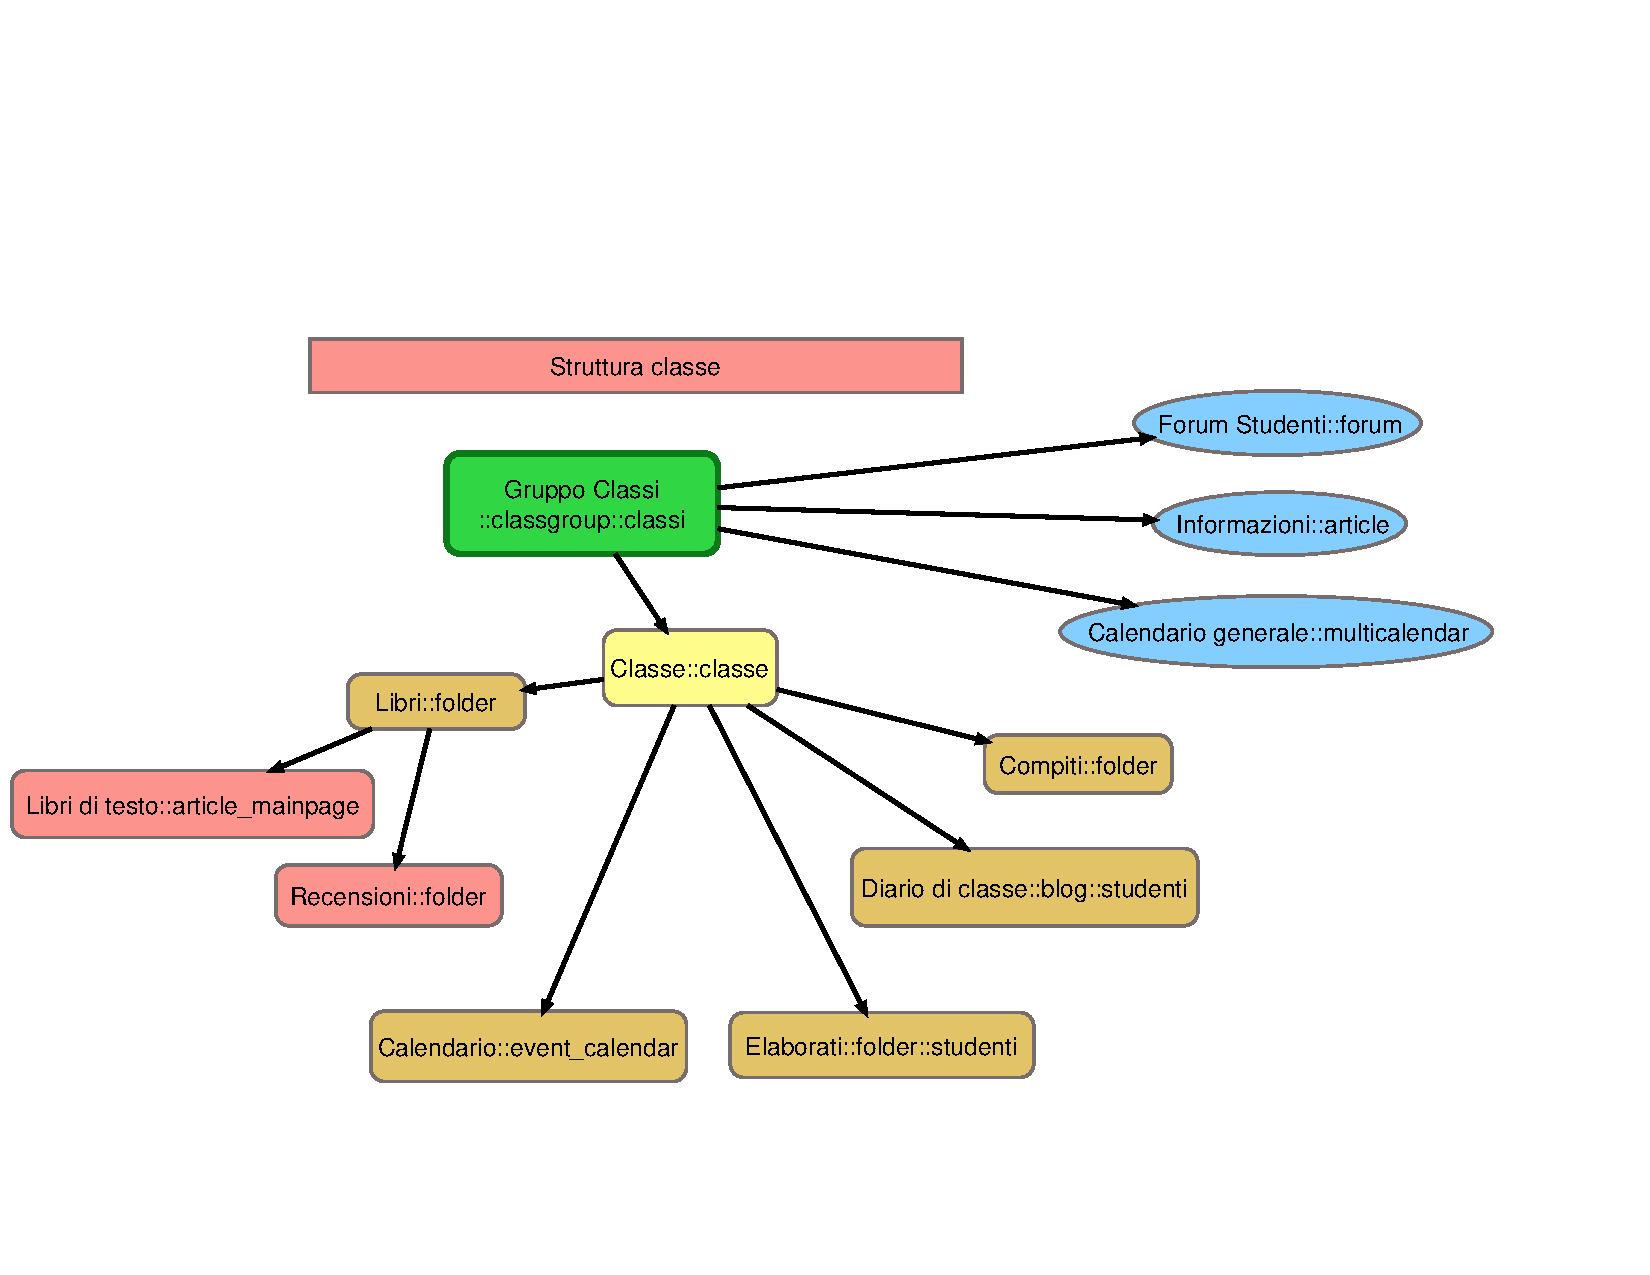
\includegraphics[width=\textwidth]{./immagini/classi/struttura_classe.png}
 % struttura_classe.png: 1455x901 pixel, 72dpi, 51.33x31.79 cm, bb=
 \caption{Struttura base della classe appena dopo la sua creazione}
 \label{fig:strut_class}
\end{figure}

\section{Classe::Commento}
Gli oggetti di questa classe rappresentano dei commenti che gli utenti possono apporre in calce agli articoli. I campi a disposizione sono:
\begin{description}
 \item[Soggetto] Il soggetto del commento
\item[Autore] L'autore del commento
\item[Messaggio]Il messaggio del commento
\end{description}

\section{Classe::Contatti}
La classe contatti deve essere utilizzata per creare delle liste di contatti del personale della scuola. Nomi, indirizzi, numeri di telefono, email etc. Un oggetto di tale classe può aggregare tutti gli oggetti della stessa classe suoi discendenti per ottenere una vista globale dei contatti. La classe Contatti consiste dei seguenti campi:

\begin{description}
 \item[Nome] Il nome esteso della pagina dei contatti
\item[Nome Breve] Il nome breve della pagina dei contatti, attenzione se lo specificate questo ha la precedenza.
\item[Aggrega contatti] Se spuntata questa voce, gli oggeti contatti figli di quello attuale verranno visualizzati nella posizione del genitore.
\item[Note]Informazioni riguardanti la pagina dei contatti
\item[Contatti esterni]Contatti riguardanti soggetti non registrati all'interno del sito
\item[Contatti interni]Contatti riguardanti soggetti registrati all'interno del sito
\end{description}

\section{Classe::Diario}
La classe diario può essere utilizzata come contenitore per brevi articoli. I contenuti in essa inseriti sono ordinati per parola chiave e data di inserimento. All'interno di un contenitore di tipo \textsl{Diario} possono essere inseriti unicamente oggetti della classe dipendente \textsl{Pagina diario}. La classe diario consiste dei seguenti campi:
\begin{description}
 \item[Nome]Il nome del contenitore es. \textsl{Diario Didattico}
\item[Descrizione] Una breve descrizione del contenuto del diario
\item[Parola chiave] Una o più parole chiave per descrivere il diario
\end{description}


\section{Classe::Dipendenti}
La classe dipendenti deve essere utilizzata per creare uno spazio in cui inserire informazioni riguardanti i dipendenti della scuola quindi Insegnanti, Personale Ata, Dsga e presidenza.I campi disponibili per questa classe sono:
\begin{description}
 \item[Nome] Il nome dell'oggetto es. \textsl{Docenti}
\item[Sommario]Un breve sommario circa i contenuti della sezione
\item[Logo]Un logo per rappresentare graficamente il gruppo di dipedenti
\item[Descrizione]Una descrizione più ampia dei contenuti della sezione
\item[Mostra oggetti figli]Visualizza gli elementi figli dell'oggetto Dipendeti
\item[Mostra extra info]Visualizza una barra laterale in cui inserire ulteriori informazioni
\end{description}


\section{Classe::Evento}
Un oggetto di questa classe deve essere obbligatoriamente contenuto da un oggetto calendario. Un oggetto evento rappresenta un entrata all'interno del calendario. È possibile specificare accadimenti sempli o con ripetizione.
I campi di questa classe sono:
\begin{description}
 \item[Titolo breve] Il titolo dell'evento visualizzato all'interno del calendario
\item[Titolo]Il titolo dell'evento mostrato nella vista completa
\item[Testo]Il testo dell'evento
\item[Categoria] La categoria a cui appartiene l'evento (tag)
\item[Da]La data di inizio dell'evento
\item[a]La data di fine dell'evento
\item[Frequenza]La frequenza di ripetizione dell'evento
\item[Fine ripetizione]Quando l'evento smette di ripetersi
\end{description}

\section{Classe::Folder}
La classe Folder deve essere utilizzata come elemento generico per la creazione di gerarchie all'interno del sisto analogamento a quanto viene fatto sul filesystem con una Directory. I campi di questa classe sono:
\begin{description}
 \item[Nome breve] Nome breve da usare nell'url e nelle viste compatte
\item[Nome]Nome del folder
\item[Icona] Icona da visualizzare nelle viste compatte
\item[Sommario]Breve introduzione dei contenuti
\item[Descrizione]Descrizione ampia dei contenuti
\item[Mostra sotto elementi]Mostra gli elementi figli
\item[Mostra extra info]Mostra una barra con ulteriori contenuti
\item[Tags]Parole chiave per descrivere i contenuti
\end{description}


\section{Classe::Folder circolari}
Il folder circolari è un elemento contenitore per le circolari emanate dalla scuola. I file contenuti all'interno di un folder circolari sono consultabile temporalmente, ovvero nella barra di destra è presente un calendario che permette all'utente di visualizzare solo quelle circolari emesse in specifi intervalli temporali.
\begin{figure}[H]
 \centering
 \includegraphics[width=\textwidth]{./immagini/classi/folder_circolari.png}
 % folder_circolari.png: 1089x236 pixel, 72dpi, 38.42x8.33 cm, bb=
 \caption{Organizzazione dei contenuti all'interno di un folder circolari}
 \label{fig:folder_circolari}
\end{figure}

I campi a disposizione di questa classe sono:
\begin{description}
 \item[Nome] Nome completo del folder
\item[Nome breve] Nome breve del folder
\item[Sommario] Sommario da mostrare nelle viste compatte
\item[Descrizione] Descrizione più dettagliata dei contenuti
\item[Logo]Logo da mostrare nelle viste compatte
\item[Tags]Parole chiave
\end{description}

\section{Classe::Folder Documenti}
Gli oggetti della classe Folder Documenti devono essere utilizzati come contenitori di file: moduli, prestampati etc. e mai come contenitori generici. I campi a disposizione di questa classe sono:
\begin{description}
\item[Nome] Il nome completo dell'unità organizzativa
\item[Nome breve]  Il nome compatto dell'unità organizzativa
\item[Icona]Un'icona per le viste compatte dell'oggetto
\item[Sommario] Un breve sommario per descrivere i contenuti del folder
\item[Mostra sotto elementi] Visualizza gli oggetti contenuti, in questo caso file e altri Folder Documenti
\item[Mostra extra info]Mostra informazioni aggiuntive sulla destra
\end{description}

\section{Classe::Formulario Feedback}
Il formulario può essere utilizzato da un utente per creare una pagina per comunicare con i visitatori del sito. Durante la creazione di un oggetto appartenente a questa classe, l'editore deve fornire un suo valido indirizzo e-mail al quale i messaggi dei visitatori saranno.
\begin{figure}[H]
 \centering
 \includegraphics[width=\textwidth]{./immagini/classi/feedback.png}
 % feedback.png: 1234x593 pixel, 72dpi, 43.53x20.92 cm, bb=
 \caption{Il creatore dell'oggetto deve fornire la sua e-mail durante la crazione del formulario per il feedback}
 \label{fig:feedback}
\end{figure}
I campi a disposizione di questa classe sono:
\begin{description}
\item[Nome] Il nome del formulario
\item[Descrizione] Una breve descrizione dello scopo del formulario
\item[Nome*]Campo che dovrà essere compilato dall'utente con il suo nome al momento dell'invio del formulario
\item[Soggetto]Il soggetto del messaggio dell'utente
\item[Messaggio] Il corpo del messaggio che l'utente vuole inviare
\item[E-mail]L'email dell'utente (se vuole essere ricontattato)
\item[E-mail destinatario]L'email di colui che crea l'oggetto. A questo indirizzo verranno inviati i messaggi scritti dagli utenti
\end{description}

\section{Classe::Forum}
La classe Forum deve essere utilizzata per creare un forum, gli oggetti di tale classe possono essere figli di un oggetto raccoglitore di forum di classe Forums. I campi a disposizione sono:
\begin{description}
\item[Nome] Il nome da assegnare al forum
\item[Descrizione] Una breve descrizione dei contenuti del forum
\end{description}

\section{Classe::Forum-argomento}
Gli oggetti di questa classe sono unicamente figli di un oggetto di classe Forum e devono essere utilizzati per creare delle discussioni all'interno  di un forum.
I campi a disposizione sono:
\begin{description}
 \item[Soggetto]L'argomento su cui verte la discussione
\item[Messaggio]Una domanda da rivolgere ai membri del forum
\item[In evidenza]L'argomento viene posto in evidenza all'interno del forum (compare tra i primi elementi)
\item[Notificami] Avvertimi se qualcuno risponde alla mia domanda
\end{description}

\section{Classe::Forum-risposta}
Gli oggetti di questa classe devono essere figli di un oggetto Forum-argomento e sono utilizzati per rispodenre alle domande che altri utenti hanno posto tramite un oggeto Forum-argomento. I campi a disposizione sono:
\begin{description}
 \item[Soggetto]Il soggetto della risposta
\item[Messaggio]Il messaggio della risposta
\end{description}

\section{Classe:Forums}
Gli oggetti di questa classe fungono da contenitori di Forum. I campi a disposizione sono:
\begin{description}
\item[Titolo]Il titolo del contenitore di forum
\item[Descrizione] Una breve descrizione dei contenuti dei forum
\end{description}

\section{Classe::Frontpage}
Gli oggetti di classe Frontpage vengono utilizzati per presentare notizie ed informazioni presenti all'interno del sito. Si rimanda al capitolo frontpage per una descrizione completa circa il loro utilizzo. I campi a disposizione sono:
\begin{description}
 \item[Nome] Il nome completo della frontpage
\item[Struttura]Il campo struttura in cui inserire le informazioni provenienti da altre sezioni del sito
\item[Etichette]Delle etichette con cui descrivere i contenuti
\end{description}

\section{Classe::Frontpage m2000}
Questa classe rappresenta un'evoluzione della classe Frontpage. Oltre al campo struttura per cui rimandiamo al capitolo sulla gestione delle frontpage è possibile inserire una descrizione in testa alla pagina, visualizzare un menu sulla sinistra e gli oggetti figli sul fondo della pagina. I campi a disposizione sono:
\begin{description}
\item[Nome] Il nome della frontpage
\item[Descrizione] Una breve descrizione dei contenuti (opzionale)
\item[Struttura]La struttura in cui inserire informazioni provenienti da altre parti del sito
\item[Etichette]Delle etichette per descrivere i contenuti
\item[Mostra menu]Visualizza o meno il menu sulla sinistra
\item[Mostra sotto elementi]Mostra gli oggetti figli
\item[Logo]Un logo da visualizzare nelle viste ridotte
\item[Piè di pagina]Testo e annotazioni da inserire nel piè di pagina
\end{description}

\section{Classe::Frontpage scuola}
Questo tipo di frontpage deve essere utilizzato per la creazione delle pagine principali di ognuna delle scuole costituenti l'istituto. I campi a disposizione sono:
\begin{description}
\item[Descrizione] Una breve descrizione della scuola che verrà posizionata in testa alla pagina
\item[Titolo]Il nome della scuola
\item[Coordinatore di sede]Il nome del coordinatore di sede
\item[Codice meccanografico]Il codice meccanografico della scuola
\item[Logo]Il logo dalla scuola come apparirà nel menu a blocchi in alto 
\item[Foto scuola]La foto della scuola
\item[Pagina]La struttura della pagina in cui pubblicare i contenuti preseti all'interno della sezione della scuola
\item[Piè di pagina]Del testo e delle note da riportare in piè di pagina
\end{description}

\section{Classe::Galleria}
Gli oggetti di questa classe devono essere utilizzati per creare gallerie di immagine e video in formato flv. I campi a disposizione sono:
\begin{description}
 \item[Nome]Il nome della galleria
\item[Breve descrizione]Una breve descrizione per le viste compatte
\item[Descrizione]Una descrizione completa per la vista totale della galleria
\item[Immagini]Un'immagine da usare come frontespizio della galleria
\item[Icona]Una piccola immagine per la visualizzazione ad icona della galleria
\item[Anno scolastico]L'anno scolastico in cui le immagini sono state fatte
\item[Mostra sotto gallerie] Visualizza le gallerie secondarie
\end{description}

\section{Classe::gruppoClassi}
Gli oggetti di questa classe fungono da aggregatori di Classi (della scuola). Vengono utilizzati per presentare l'insieme di tutte le classi del corrente anno scolastico di ogni scuola. I campi a disposizione sono:
\begin{description}
\item[Nome]Il nome del gruppo di classi
\item[Nome breve]Un nome breve da mostrare nelle viste compatte e nell'url
\item[Sommario]Un breve sommario da mostrare nelle viste compatte
\item[Descrizione]La descrizione delle classi della scuola
\item[Mostra extra info]Se mostrare  o meno una barra a destra con informazioni aggiuntive
\item[Tags]Etichette che descrivono il contenuto
\end{description}

\section{Classe::gruppoDocenti}
Gli oggetti di tale classe vengono utilizzati come raccoglitori degli spazi personali dei docenti. I campi a disposizione sono:
\begin{description}
 \item[Nome]Il nome del gruppo di docenti
\item[Nome breve]Un nome breve da mostrare nelle viste compatte
\item[Sommario]Il sommario da mostrare nelle viste compatte
\item[Descrizione]Un descrizione più completa da mostrare nelle viste totali
\end{description}

\section{Classe::Colonna info}
Gli oggetti di questa classe possono essere utilizzati per fornire in una colonna sulla destra dei contenuti delle informazioni aggiuntive. Si rimanda al capitolo ad esse dedicato per ulteriori informazioni. I campi a disposizione sono:
\begin{description}
 \item[Titolo] Il nome della colonna di informazioni
\item[Immagine] Un'immagine con cui aprire la colonna
\item[Url immagine] Un link da associare all'immagine
\item[Contenuto] Il testo delle informazioni aggiuntive che si vogliono dare
\item[Url] Un link da associare alle informazioni
\end{description}

\section{Classe:Layout Globale}
Gli oggetti di questa classe possono essere utilizzati per fornire in una colonna sulla destra dei contenuti delle informazioni aggiuntive. Si rimanda al capitolo ad esse dedicato per ulteriori informazioni. I campi a disposizione sono:
\begin{description}
 \item[Nome]Il nome della colonna di informazioni
\item[Blocchi] Colonna per pubblicare contenuti correlati
\end{description}

\section{Classe::Libro}
Gli oggetti di questa classe rappresentano dei libri e possono essere utilizzati per, ad esempio, inserire i libri della biblioteca scolastica. I campi a disposizione sono:
\begin{description}
\item[Titolo]Il titolo del libro
\item[Autore]L'autore o gli autori separati da una virgola del libro
\item[Casa editrice]La casa editrice del libro
\item[Copertina]Un'immagine della copertina del libro
\item[Descrizione]Descrizione del libro
\item[Isbn]Il codice isbn del libro
\end{description}

\section{Classe::Link}
Gli oggetti di questa classe vengono utilizzati per creare dei collegamenti a risorse esterne al sito es. il sito del ministero della pubblica istruzione. I campi a disposizione sone:
\begin{description}
 \item[Nome] Il nome del link
\item[Descrizione] Una breve descrizione delle risorse raggiungibili seguendo il link
\item[Indirizzo]L'url del link
\end{description}

\section{Classe::Macroarea}
Gli oggetti di questo tipo fungono da frontpage per le macroare. Un oggetto di tipo Frontpage dovrebbe contenere unicamente oggetti di tipo Frontpage. I campi disponibili sono:
\begin{description}
 \item[Titolo]Il nome della macroarea
\item[Descrizione]Una descrizione dei contenuti della zona
\item[Pagina]Un elemento contenitore di blocchi per il cui utilizzo rinviamo alla sezione frontpage
\item[Logo]Un'immagine da mostrare nella vista ad icone 
\item[Referente]Il referente della macroarea da selezionare tra gli iscritti al sito
\item[Mostra menu]Se mostrare o meno il menu sulla sinistra
\item[Mostra figli]Se mostrare o meno gli oggetti figli
\end{description}

\section{Classe::Pagina diario}
Gli oggetti di questa classe rappresentano dei brevi articoli che andranno a costituire le pagine di un diario. Tali oggetti potranno essere unicamente figli di un padre di classe Diario. Le classi Diario e Pagina diario sono quindi utilizzate per cotruire l'analogo di un \textsl{Blog}. I campi a disposisizione sono:
\begin{description}
 \item[Titolo] Il titolo della pagine di diario
\item[Corpo] Il corpo del testo
\item[Data di pubblicazione] La data in cui il contenuto verrà reso pubblicamente disponibile
\item[Data di de pubblicazione]La data in cui il contenuto non sarà più pubblicamente disponibile
\item[Parole chiave]Le parole chiave da associare al contenuto
\item[Abilita commenti] Campo per abilitare la possibilità di commentare il contenuto.
\end{description}

\section{Classe::Professore (spazio personale)}
Gli oggetti di questa classe vengono creati automaticamente durante il processo di registrazione di un insegnate. Essi rappresentano dei contenitori all'interno dei quali i docenti potranno caricare i propri materiali didattici. Per una descrizione più approfondita rimandiamo al capitolo correlato. I campi a disposizione sono:
\begin{description}
\item[Nome]Il nome del docente (auto assegnato durante la creazione dell'account)
\item[Nome breve]Un nome breve da usare nelle viste compatte
\item[Telefono]Il numero di telefono del docente
\item[Email]L'email del docente (distinta o uguale a quella di registrazione)
\item[Ruolo]Il ruolo del docente: vicepreside, collaboratore etc.
\item[Descrizione]Una descrizione del docente
\item[Mostra sotto elementi]Se mostrare o meno i contenuti figli in calce
\item[Tags]Delle etichette per categorizzare il docente
\end{description}

\section{Classe::Progetto}
Gli oggetti di questa classe devono essere utilizzati per creare un contenitore per i progetti e devono essere preferibilmente inseriti in un Folder. I campi a disposizione sono:
\begin{description}
 \item[Titolo] Il titolo completo del progetto
\item[Titolo breve] Un titolo breve per il progetto da mostrare nelle viste compatte
\item[Docenti responsabili] I docenti responsabili del progetto da selezionare tra i docenti registrati
\item[Codice progetto] Il codice del progetto fornito dalla segreteria
\item[Autore] L'autore del contenuto
\item[Introduzione]Breve introduzione del progetto da mostrare nelle viste compatte
\item[Corpo]Il corpo del testo del progetto
\item[Logo]Il logo del progetto per le viste compatte
\item[Mostra figli]Se mostrare gli oggetti figli dell'oggetto contenitore progetto
\item[Parola chiave]Una o più parole chiave per descrivere i contenuti del progetto
\end{description}

\section{Classe::Questionario (breve)}
Classe per creare dei sondaggi breve (una singola domanda). Tali oggetti possono essere inseriti, ad esempio, nella pagina principale del sito. I campi a disposizione sono:
\begin{description}
\item[Nome]Il nome del sondaggio breve
\item[Descrizione]La descrizione del sondaggio
\item[Domanda]Il testo della domanda
\end{description}

\section{Classe::Raccoglitore circolari}
Gli oggetti di questa classe sono utilizzati come contenitori di oggetti del tipo Folder Circolari. I campi a disposizione sono:
\begin{description}
\item[Nome] Il nome del direttorio per le circolari
\item[Nome Breve]Un nome breve da utilizzare nelle viste compatte
\item[Sommario]Un sommario da mostrare nelle viste compatte
\item[Descrizione]La descrizione per le viste totali
\item[Mostra extra info]Se mostrare o meno una barra sulla destra con ulteriori informazioni
\item[Tags]Delle etichette per categorizzare il contenuto.
\end{description}

\section{Classe::Sondaggio}
Gli oggetti di questa classe sono utilizzati per creare sondaggi complessi. Per una descrizione approfondita del loro utilizzo rimandiamo al capitolo corrispondente. I campi a disposizione sono:
\begin{description}
\item[Nome]Il nome del sondaggio
\item[Logo]Un'immagine da mostrare nelle viste compatte e nella vista totale
\item[Descrizione]Un breve descrizione del sondaggio
\item[Sondaggio]Il sondaggio multi domanda
\end{description}

\section{Classe::Ufficio}
Gli oggetti di questa classe vengono usati per rappresentare gli uffici della scuola. 
\begin{description}
\item[Nome] Il nome dell'ufficio
\item[Responsabile ufficio]Il nome del responsabile dell'ufficio
\item[Logo]Un'immagine per le viste ad icona
\item[Attività ufficio]Il tipo di attività dell'ufficio
\item[Contatti ufficio] I contatti del personale dell'ufficio
\item[In evidenza]Gli elementi in evidenza, campo a blocchi	
\end{description}




\chapter[Interfaccia modifica]{Interfaccia per la modifica dei contenuti}


Il cms scolastico basato su EzPublish permette di modificare agevolmente i contenuti creati e di mantenere una storia delle modifiche effettuate. Nell'attuale implementazione vengono conservate, per motivi di spazio, unicamente due copie di un oggetto presente nell'albero dei contenuti.
\begin{figure}[H]
 \centering
 \includegraphics[width=0.7\textwidth]{./immagini/edit/revisioni.png}
 % revisioni.png: 1042x621 pixel, 200dpi, 13.23x7.88 cm, bb=
 \caption{Per ogni oggetto è presente lo stato (n-1)-esimo lo stato ennesimo e la bozza creata al momento della modifica}
 \label{fig:revisioni}
\end{figure}

Quando l'utente inizia a modificare un oggetto viene automaticamente creata una bozza dello stesso sulla quale si andrà ad operare lasciando intatta la versione precedente del contenuto. L'utente può in qualsiasi momento decidere di scartare la bozza e tornare alla versione precedente del documento, di salvare la bozza senza pubblicarla oppure di pubblicarla eliminando la versiona (n-1)esima 
\section{Gestione delle revisioni}
Tramite il backend amministrativo è possibile gestire le versioni di un oggetto. Il link per la modifica delle revisioni è disponibile in modalità modifica tramite il pulsante \includegraphics[bb=0 0 261 36]{./immagini/edit/tasto_versioni.png}.
\begin{figure}[H]
 \centering
 \includegraphics[width=\textwidth,bb=0 0 1237 528]{./immagini/edit/gestione_revisioni.png}
 % gestione_revisioni.png: 1237x528 pixel, 72dpi, 43.64x18.63 cm, bb=0 0 1237 528
 \caption{Interfaccia per la modifica delle revisioni}
 \label{fig:gestione_revisioni}
\end{figure}


\section{Barre degli strumenti}

Gli utenti con sufficienti permessi dopo aver effettuato il login sono in grado di accedere alla barra di modifica/aggiunta contenuti fig.\ref{fig:edit_ext}. È possibile creare, modificare o eliminare gli oggetti presenti nell'albero dei contenuti. In funzione del gruppo cui appartiene l'utente i contenuti modificati/creati saranno immediatamente visibili oppure soggetti ad approvazione da parte di utenti con privilegi maggiori.

\subsection{Barra degli strumenti principale}

La barra degli strumenti principale è visibile su ogni pagina del sito dopo aver effettuato il login e permette agli utenti di interagire con i contenuti. L'insieme di azioni permesse sarà determinato dalle autorizzazioni di cui ogni utente gode.

\begin{figure}[H]
 \centering
 \includegraphics[width=\textwidth]{./immagini/edit/barra_edit_esterna.png}
 % barra_edit_esterna.png: 571x32 pixel, 72dpi, 20.14x1.13 cm, bb=
 \caption{Barra per la modifica dei contenuti: vista contenuto}
 \label{fig:edit_ext}
\end{figure}

\begin{figure}[H]
\begin{center}
\begin{tabular}{m{0.1\textwidth}l}
\includegraphics[bb=0 0 25 32]{./immagini/edit/tasto_add.png}& Tasto aggiungi oggetto\\
\includegraphics[bb=0 0 261 36]{./immagini/edit/tasto_modifica.png}& Tasto modifica oggetto\\
\includegraphics[bb=0 0 26 32]{./immagini/edit/tasto_sposta.png}& Tasto sposta nodo\\
\includegraphics[bb=0 0 26 32]{./immagini/edit/tasto_canc.png}& Tasto cancella oggetto\\
\includegraphics[bb=0 0 26 32]{./immagini/edit/tasto_ordina.png}& Tasto cambia ordinamento elementi\\
\includegraphics[bb=0 0 26 32]{./immagini/edit/tasto_stato.png}& Tasto cambia stato dell'oggetto\\
\includegraphics[bb=0 0 26 32]{./immagini/edit/tasto_coll.png}& Tasto aggiungi collocazioni per l'oggetto\\
\includegraphics[bb=0 0 26 32]{./immagini/edit/tasto_cache.png}& Tasto cancella la cache dell'oggetto
\end{tabular}
\caption{I pulsanti presenti nella barra per l'interazione con i contenuti)}
\end{center}
\end{figure}


\subsection{Barre degli strumenti secondaria}

Dopo essere entrati in modalità modifica oggetto la barra degli strumenti cambia per permetterci di gestire le proprietà interne dell'oggetto fig.\ref{fig:edit_intern}:

\begin{figure}[H]
 \centering
 \includegraphics[width=\textwidth]{./immagini/edit/barra_edit_interna.png}
 % barra_edit_interna.png: 274x35 pixel, 72dpi, 9.67x1.23 cm, bb=
 \caption{Barra modifica: vista modifica oggetto}
 \label{fig:edit_intern}
\end{figure}

\begin{center}
\begin{tabular}{m{0.1\textwidth}l}
\includegraphics[bb=0 0 25 32]{./immagini/edit/tasto_pubblica.png}& Salva l'oggetto modificato e pubblicalo immediatamente\\
\includegraphics[bb=0 0 261 36]{./immagini/edit/tasto_versioni.png}& Gestisci le versioni dell'oggetto\\
\includegraphics[bb=0 0 26 32]{./immagini/edit/tasto_esci.png}& Salve ed esci\\
\includegraphics[bb=0 0 26 32]{./immagini/edit/tasto_anteprima.png}& Mostra un'anteprima delle modifiche correnti\\
\includegraphics[bb=0 0 26 32]{./immagini/edit/tasto_traduci.png}& Traduci il testo in una delle lingue disponibili
\end{tabular}
\end{center}



\section{Editor Xml}

Ezpublish ci mette a disposizione un  editor di testo basato su TinyMce per l'inserimento di articoli all'interno del database. Quando copiamo del testo all'interno dell'area attiva questo viene trasformato in Xml e quindi reso disponibile all'utente per ulteriori modifiche. L'editor dispone di tutte le caratteristiche standard di un Editor di testi. Quando andrete a modificare i contenuti dovreste rispettare queste regole:
\begin{itemize}
\item Cercate di formattare il testo in accordo al tema generale del sito
\item Non utilizzate un eccesso di formattazione (sfondi, maiuscole, colori etc.)
\item Non fate copia e in colla dal vostro editor di testo preferito di documenti eccessivamente complessi. L'editor di testo presente all'interno del sito non è stato creato per gestire libri o documenti di grandi dimensioni.
\end{itemize}

\begin{figure}[H]
 \centering
 \includegraphics[width=\textwidth]{./immagini/edit/barra_ezoe.png}
 % barra_ezoe.png: 988x27 pixel, 72dpi, 34.85x0.95 cm, bb=
 \caption{Barra degli strumenti dell'editor di testo xml}
 \label{fig:ezoe_barra}
\end{figure}

\begin{figure}[H]
 \centering
 \includegraphics[width=\textwidth]{./immagini/edit/ezoe.png}
 % ezoe.png: 992x170 pixel, 72dpi, 35.00x6.00 cm, bb=
 \caption{Interfaccia dell'editor di testo XML}
 \label{fig:ezoe_finestra}
\end{figure}

\Ovalbox{%
\begin{minipage}{0.8\textwidth}
\bf Trascinando l'angolo in basso a destra della cornice dell'editor di testo è possibile ingrandire l'area di modifica del testo
\end{minipage}}



\section[Embedding contenuti]{Inserimento di elementi contenuto all'interno del testo}

Uno dei grandi pregi del cms utilizzato è rappresentato dalla possibilità di utilizzare qualsiasi elemento già pubblicato all'interno di un campo xml, ovvero all'interno della finestra dell'editor di testo. Potete inserire, foto, articoli, file etc. Oltre all'inserimento di materiali già caricati è possibile, direttamente dall'interfaccia di modifica, inserire nuovi contenuti come file e immagini. Durante il caricamento di materiali da associare agli articoli è importante scegliere la collocazione più appropriata tra quelle suggerite figura.\ref{fig:edit_scelta_collocazione}

\begin{figure}[H]
 \centering
 \includegraphics[width=0.6\textwidth]{./immagini/edit/scelta_collocazione.png}
 % scelta_collocazione.png: 513x429 pixel, 90dpi, 14.48x12.11 cm, bb=
 \caption{Scelta delle collocazione per l'immagine da caricare}
 \label{fig:edit_scelta_collocazione}
\end{figure}

in questo modo potremo poi riutilizzare i materiali caricati per altri articoli/contenuti. Se l'utente ha a disposizione uno spazio personale questo sarà automaticamente elencato tra le possibili collocazioni dei contenuti.
I passaggi per caricare un file/immagine all'interno del sito sono quindi:
\begin{itemize}
 \item Cliccare sul link appropriato nella barra degli strumenti dell'editor di testo
\item Compare la finestra di dialogo figura.\ref{fig:load_image}
\item Inseriamo i dati richiesti figura.\ref{fig:caricamento_immagine}
  \begin{itemize}
  \item il nome dell'immagine
   \item il file da caricare
  \item la collocazione del file
  \item il testo alternativo da visualizzare in browser testuali
  \item La discalia dell'immagine
  \end{itemize}
\end{itemize}


\begin{figure}[H]
 \centering
 \includegraphics[width=0.6\textwidth]{./immagini/edit/carica_immagine.png}
 % carica_immagine.png: 510x428 pixel, 72dpi, 17.99x15.10 cm, bb=
 \caption{Interfaccia per il caricamento di un'immagine locale}
 \label{fig:load_image}
\end{figure}


\begin{figure}[H]
 \centering
 \includegraphics[width=0.6\textwidth]{./immagini/edit/caricamento_immagine.png}
 % caricamento_immagine.png: 476x198 pixel, 72dpi, 16.79x6.99 cm, bb=
 \caption{Dati da inserire durante il caricamento di una immagine}
 \label{fig:caricamento_immagine}
\end{figure}

Oltre a caricare nuove immagini possiamo utilizzare elementi precedentemente caricati carcandoli all'iterno dell'albero dei contenuti figura.\ref{fig:cerca_immagine}

\begin{figure}[H]
 \centering
 \includegraphics[width=0.6\textwidth]{./immagini/edit/cerca_immagine.png}
 % cerca_immagine.png: 511x427 pixel, 72dpi, 18.03x15.06 cm, bb=
 \caption{Interfaccia per la ricerca di un'immagine precedentemente inserita}
 \label{fig:cerca_immagine}
\end{figure}

l'inserimento di file è del tutto analogo a quanto ora sposto circa le immagini. L'inserimento di un oggetto di contenuto generico all'interno del testo è analogo a quanto fatto per  un'immagine già caricata figura.\ref{fig:embed_ogg}


\begin{figure}[H]
 \centering
 \includegraphics[width=\textwidth]{./immagini/edit/embed_oggetto.png}
 % embed_oggetto.png: 508x488 pixel, 72dpi, 17.92x17.22 cm, bb=
 \caption{Nello stesso modo in cui possiamo inserire delle immagine all'interno del testo è possible inserire un qualsiasi elemento del sito}
 \label{fig:embed_ogg}
\end{figure}

\section{Modifica degli elementi del testo}

L'editor di test ci permette di modificare agevolmente ogni elemento presente all'interno della finestra di modifica. È sufficiente cliccare con il mouse sull'elemento che vogliamo modificare, nella barra inferiore della finestra dell'editor comparirà il nome della classe dell'elemento e la sua relazione di parentela figura.\ref{fig:ezoe_mod}

\begin{figure}[H]
 \centering
 \includegraphics[width=0.6\textwidth]{./immagini/edit/ezoe_modifica_embed.png}
 % ezoe_modifica_embed.png: 220x24 pixel, 72dpi, 7.76x0.85 cm, bb=
 \caption{Quando selezioniamo un elemento all'interno del test, sulla barra di stato dell'editor compare la classe dell'elemento selezionato}
 \label{fig:ezoe_mod}
\end{figure}

Se clicchiamo sul nome della classe dell'elemento possiamo accedere all'interfaccia di modifica delle proprietà del tag se ad esempio clicchiamo su un oggetto inserito (embedded) comparirà una finestra come quella di figura.\ref{fig:edit_image}


\begin{figure}[H]
 \centering
 \includegraphics[width=0.8\textwidth]{./immagini/edit/modifica_immagine.png}
 % modifica_immagine.png: 506x486 pixel, 72dpi, 17.85x17.15 cm, bb=
 \caption{Modifica proprietà immagine}
 \label{fig:edit_image}
\end{figure}


se clicchiamo su una tabella figura.\ref{fig:edit_tabella}


\begin{figure}[H]
 \centering
 \includegraphics[width=0.6\textwidth]{./immagini/edit/edit_tabella.png}
 % edit_tabella.png: 441x199 pixel, 72dpi, 15.56x7.02 cm, bb=
 \caption{Modifica di una tabella}
 \label{fig:edit_tabella}
\end{figure}

\chapter[Sondaggi]{Gestione dei sondaggi}

Tramite il CMS è possibile creare dei sondaggi, da sottoporre agli utenti registrati e non. L'editore con i permessi per la creazione di un sondaggio procede alla stregue di qualsiasi altro contenuto. Dalla barra degli strumenti sceglie la classe sondaggio e tramite il pulsante di creazione istanzia un oggetto di tipo sondaggio. I sondaggi dovrebbero essere contenuti all'interno di un oggetto di classe Folder. L'editore dovrà inserire il nome del sondaggio, un'immagine che verrà visualizzata durante le viste compatte e tanti elementi di tipo domanda quanti ne seranno richiesti. Le domande possibili sono:
\begin{description}
 \item[Section Header/Intestazione sezione] Inserite una stringa di testo per separare sezioni semanticamente distinte del questionario (attenzione questa tipo di domanda non ammette risposte)
\item[Paragraph/paragrafo]Inserite un paragrafo per illustrare il significato delle domande.
\item[Scelta singola/multipla]Domanda a scelta multipla standard, è possibile inserire un campo per permettere all'utente una risposta personalizzata
\item[Text entri/Inserimento testo]Domanda aperta
\item[Number entry]Domanda la cui risposta sarà un numero intero o razionale
\item[Related object/Oggetto correlato] Un oggetto con un campo xml, può essere usato per illustrare delle domande con immagini, testo formattato etc.
\item[Form Receiver/Ricevente]Inserite l'email dell'utente che riceverà \textbf{tutti} i risultati delle votazioni. Per ogni votazione verrà quindi inviata un'email a tale utente.
\item[Group password/Password di gruppo]Password per l'inserimento pubblico. Quando viene creato un questionario con una domanda di questo tipo gli utenti dovranno inserire la password creata dall'editore il quale può stabilire il numero massimo di volte per cui è possibile votare.
\end{description}

\section{Creazione del sondaggio}


\begin{figure}[H]
 \centering
 \includegraphics[width=\textwidth]{./immagini/survey/survey_immagine.png}
 % survey_immagine.png: 1241x542 pixel, 72dpi, 43.78x19.12 cm, bb=
 \caption{Durante la creazione di un sondaggio è possibile caricare un'immagine che verrà mostrata anche nelle viste compatte}
 \label{fig:survey_imm}
\end{figure}
 Inserire un'immagine come mostrate in figura.\ref{fig:survey_imm} può essere molto utile per aumentare la visibilità del sondaggio nelle viste compatte ad esempio nella pagina principale del sito.

\begin{figure}[H]
 \centering
 \includegraphics[width=\textwidth,bb=0 0 1256 227]{./immagini/survey/surver_descr.png}
 % surver_descr.png: 1256x227 pixel, 72dpi, 44.31x8.01 cm, bb=0 0 1256 227
 \caption{Campo di testo per la descrizione del sondaggio}
 \label{fig:survey_descr}
\end{figure}
Dovreste scrivere una breve descrizione per ogni sondaggio per spiegare all'utente le modalità di votazione e il sistema con cui verranno elaborati i dati.
\begin{figure}[H]
 \centering
 \includegraphics[width=\textwidth]{./immagini/survey/survey_prop.png}
 % survey_prop.png: 1237x289 pixel, 72dpi, 43.64x10.20 cm, bb=
 \caption{Opzioni generali del sondaggio}
 \label{fig:survey_opzioni}
\end{figure}

Durante la creazione del sondaggio è possibile specificare alcuni importanti parametri come si può vedere in figura.\ref{fig:survey_opzioni} analiziamoli insieme:
\begin{description}
 \item[Abilitato] È possibili disabilitare manualmente un sondaggio, gli utenti non potranno quindi più votare fino a che l'editore non avrà riabilitato il sondaggio
\item[Pui dare solo un'unica risposta] L'utente potrà dara un'unica risposta che non potrà più essere modificata il questionario sarà unicamente disponibile unicamente per gli utenti registrati.
\item[Inserimento dell'utente persistente]L'utente potrà modificare in un secondo momento  la sua votazione, attenzione non selezionate questa opzione insieme alla precedente in quanto la votazione unica avrà la precedenza.
\item[Attivo da]Il questionario sarà utilizzabile dagli utenti dalla data indicata
\item[Attivo fino a] alla data indicata
\end{description}

\begin{figure}[H]
 \centering
 \includegraphics[width=\textwidth]{./immagini/survey/survey_multiop.png}
 % survey_multiop.png: 1237x361 pixel, 72dpi, 43.64x12.74 cm, bb=
 \caption{Domanda a scelta multipla}
 \label{fig:survey_multiop}
\end{figure}

\begin{figure}[H]
 \centering
 \includegraphics[width=\textwidth]{./immagini/survey/survey_password.png}
 % survey_password.png: 1249x258 pixel, 72dpi, 44.06x9.10 cm, bb=
 \caption{Survey pubblica con password di gruppo}
 \label{fig:survey_pwd}
\end{figure}

Tramite l'utilizzo di una password di gruppo sarà possibile creare questionari totalmente anonimi rivolti a gruppi di utenti figura.\ref{fig:survey_pwd}

\begin{figure}[H]
 \centering
 \includegraphics[width=\textwidth]{./immagini/survey/survey_view.png}
 % survey_view.png: 1065x567 pixel, 72dpi, 37.57x20.00 cm, bb=
 \caption{Vista pubblica del sondaggio}
 \label{fig:survey_view}
\end{figure}


\section{Analisi dei risultati}

Gli editori e tutti gli utenti con accesso al backend del sito potranno accedere al pannello per l'analisi dei dati disponibile dal menu \textbf{Survey} nella barra principale. Qui compariranno tutti i questionari presenti nel sito figura.\ref{fig:survey_list}

\begin{figure}[H]
 \centering
 \includegraphics[width=\textwidth]{./immagini/survey/elenco_questionari.png}
 % elenco_questionari.png: 908x136 pixel, 72dpi, 32.03x4.80 cm, bb=
 \caption{Elenco dei questionari presenti nel sito}
 \label{fig:survey_list}
\end{figure}

Cliccando sul pulsante con l'istogramma accederete alla statista delle votazioni  figura.\ref{survey_votes}

\begin{figure}[H]
 \centering
 \includegraphics[width=\textwidth]{./immagini/survey/sondaggio_risultati.png}
 % sondaggio_risultati.png: 904x305 pixel, 72dpi, 31.89x10.76 cm, bb=
 \caption{La statistica delle votazioni del sondaggio}
 \label{fig:survey_votes}
\end{figure}

per effettuare ulteriori elaborazioni sui dati raccolti il sistema mette a disposizione dell'utente una comoda esportazione in formato CSV dei dati.






\chapter[Revisione]{Come approvare i contenuti prodotti dagli utenti}

%\begin{landscape}
\begin{figure}[H]
 \centering
 \includegraphics[width=\textwidth]{./immagini/chapter_approval/revisione.pdf}
 % approve_workflow1.png: 928x176 pixel, 72dpi, 32.74x6.21 cm, bb=
 \caption{Flusso per l'approvazione di un contenuto}
 \label{fig:approve_workflow1}
\end{figure}
%\end{landscape}

\section{Esempio di approvazione}

Il cms scolastico  mette a disposizione degli editori un sistema per la revisione dei contenuti prima che questi siano approvati. Un piccolo esempio ci permetterà di capire come funziona il sistema per la revisione. Immagineremo che uno studente \textsl{Gianni} sia stato incaricato da un suo insegnante \textsl{Prof. Matematica} di creare un articolo all'interno dello spazio riservato alla sua clase.
Gianni crea quindi un articolo nello spazio riservato alla 5B e lo pubblica. Siccome Gianni è un utente  i cui permessi non sono sufficienti per la pubblicazione immediata viene inviato alla pagina di selezione dei revisori fig.\ref{fig:approve_select1}
\begin{figure}[H]
 \centering
 \includegraphics[width=\textwidth]{./immagini/chapter_approval/approve_select1.png}
 % approve_select1.png: 1264x249 pixel, 72dpi, 44.59x8.78 cm, bb=
 \label{fig:approve_select1}
\end{figure}
Cliccando su aggiungi utenti Gianni potrà selezionare il Prof. di Matematica, quando Gianni sottoporrà a revisione altri articoli tutti i revisori precedenti saranno ricordati in modo da permettere un più celere processo di approvazione fig.\ref{fig:approve_select10}
\begin{figure}[H]
 \centering
 \includegraphics[width=\textwidth]{./immagini/chapter_approval/approve_select10.png}
 % approve_select1.png: 1264x249 pixel, 72dpi, 44.59x8.78 cm, bb=
\caption{Durante un successivo processo di approvazione i precedenti revisori sono automaticamente resi disponibili} 
\label{fig:approve_select10}
\end{figure}

\begin{figure}[H]
 \centering
 \includegraphics[width=\textwidth]{./immagini/chapter_approval/approve_select2.png}
 % approve_select1.png: 1264x249 pixel, 72dpi, 44.59x8.78 cm, bb=
\caption{Gianni selezione il revisore scorrendo la lista degli utenti}  
\label{fig:approve_select2}
\end{figure}

Dopo aver selezionato il revisore e continuato il flusso di lavoro Gianni può inviare un messaggio al suo revisore circa possibili problemi che quest ultimo potrebbe incontrare.
\begin{figure}[H]
 \centering
 \includegraphics[width=\textwidth]{./immagini/chapter_approval/approve_select3.png}
 % approve_select1.png: 1264x249 pixel, 72dpi, 44.59x8.78 cm, bb=
\caption{Dopo aver selezionato il revisore questo compare nella lista degli utenti revisori del contenuto appena pubblicato}
\label{fig:approve_select3}
\end{figure}

Il messaggio sarà reso disponibile all'utente revisore che potrà comunicare con Gianni attraverso l'interfaccia di approvazione.

\begin{figure}[H]
 \centering
 \includegraphics[width=\textwidth]{./immagini/chapter_approval/approve_select4.png}
 % approve_select1.png: 1264x249 pixel, 72dpi, 44.59x8.78 cm, bb=
\caption{Gianni può mandare un messaggio all'utente revisore}
\label{fig:approve_select4}
\end{figure}

Gianni potrà monitorare lo stato dei suoi articoli nella sua area riservata (\textsl{Il mio profilo}) 

\begin{figure}[H]
 \centering
 \includegraphics[width=\textwidth]{./immagini/chapter_approval/approve_select5.png}
 % approve_select1.png: 1264x249 pixel, 72dpi, 44.59x8.78 cm, bb=
\caption{Stato dell'articolo appena pubblicato} 
\label{fig:approve_select5}
\end{figure}

\begin{figure}[H]
 \centering
 \includegraphics[width=\textwidth]{./immagini/chapter_approval/approve_select6.png}
 % approve_select1.png: 1264x249 pixel, 72dpi, 44.59x8.78 cm, bb=
\caption{L'articolo appena creato da Gianni attende di essere approvato o respinto} 
\label{fig:approve_select6}
\end{figure}

L'utente revisore, in questo caso il Prof. di Matematica riceve nella sua area personale (e via e-mail) un avviso circa il nuovo contenuto in attesa di approvazione. Il Prof. di Matematica entra nella sua area personale e dal menu \textsl{Collaborazione} vede il contenuto creato da Gianni:

\begin{figure}[H]
 \centering
 \includegraphics[width=\textwidth]{./immagini/chapter_approval/approve_select7.png}
 % approve_select1.png: 1264x249 pixel, 72dpi, 44.59x8.78 cm, bb=
 \label{fig:approve_select7}
\end{figure}

Cliccando sulla voce nel menu Collaborazione il Prof. può vedere un'anteprima del lavoro di Gianni e decidere se:
\begin{itemize}
 \item Approvare il contenuto
\item Modificare il contenuto ed approvarlo
\item Rimandare il contenuto a Gianni affinchè questo lo modifichi
\end{itemize}
\begin{figure}[H]
 \centering
 \includegraphics[width=\textwidth]{./immagini/chapter_approval/approve_select8.png}
 % approve_select1.png: 1264x249 pixel, 72dpi, 44.59x8.78 cm, bb=
 \label{fig:approve_select8}
\end{figure}

Se il contenuto è stato approvato  dopo circa 5 minuti sarà disponibile nella zona pubblica del sito.
\begin{figure}[H]
 \centering
 \includegraphics[width=\textwidth]{./immagini/chapter_approval/approve_select9.png}
 % approve_select1.png: 1264x249 pixel, 72dpi, 44.59x8.78 cm, bb=
\caption{Il sistema notifica la avvenuta approvazione del contenuto} 
\label{fig:approve_select9}
\end{figure}

\section{Creazione del Workflow}

Per abilitare il sistema di approvazione è necessario creare dal backend amministrativo un workflow, ovvero un insieme di azioni da intraprendere sul contenuto quando una determinata condizione è soddisfatta. Dal menu impostazioni scegliamo Workflow ed entramo nella collezione standard di workflow:
\begin{figure}[H]
 \centering
 \includegraphics[width=\textwidth]{./immagini/chapter_approval/approve_workflow1.png}
 % approve_workflow1.png: 928x176 pixel, 72dpi, 32.74x6.21 cm, bb=
 \caption{Per abilitare l'approvazione dei contenuti è necessario creare un oggetto all'interno della catena dei flussi di lavoro}
 \label{fig:approve_workflow2}
\end{figure}
Creiamo quindi un workflow che verrà eseguito ogni volta che un utente di un particolare gruppo pubblica un contenuto:

\begin{figure}[H]
 \centering
 \includegraphics[width=\textwidth]{./immagini/chapter_approval/approve_workflow_create.png}
 % approve_workflow_create.png: 930x350 pixel, 72dpi, 32.81x12.35 cm, bb=
 \caption{Una volta selezionato il gruppo di workflow di interesse dobbiamo creare un nuovo workflow}
 \label{fig:approve_create}
\end{figure}
Per il workflow di approvazione descritto nell'esempio precedente selezioniamo l'evento Revisione Avanzata:

\begin{figure}[H]
 \centering
 \includegraphics[width=\textwidth]{./immagini/chapter_approval/approve_workflow_creation.png}
 % approve_workflow_creation.png: 928x265 pixel, 72dpi, 32.74x9.35 cm, bb=
 \caption{Durante la creazione del workflow per l'approvazione dobbiamo selezionare quali eventi intendiamo inserire}
 \label{fig:approve_create1}
\end{figure}

Nel interfaccia di modifica/creazione ci viene chiesto di inserire alcuni parametri:
\begin{figure}[H]
 \centering
 \includegraphics[width=\textwidth]{./immagini/chapter_approval/approve_workflow_edit1.png}
 % approve_workflow_edit1.png: 924x564 pixel, 72dpi, 32.60x19.90 cm, bb=
 \caption{L'evento revisione avanzata mette a disposizione due modalità: approvazione con revisori preselezionati e approvazione con revisori selezionati dagli utenti}
 \label{fig:approve_edit1}
\end{figure}

\begin{description}
 \item[Sezioni interessate] Le sezioni del sito soggette ad approvazione, nell'esempio la sezione Alunni
\item[Sistema di revisione]È possibile scegliere tra una lista predefinita di Revisori oppure lasciare la scelta all'utente come nell'esempio
\item[Gruppi di utenti esclusi]Gli utenti appartenenti a questi gruppi possono sempre pubblicare istantaneamente i contenuti
\end{description}



\begin{figure}[H]
 \centering
 \includegraphics[width=\textwidth]{./immagini/chapter_approval/approve_workflow_edit2.png}
 % approve_workflow_edit2.png: 928x544 pixel, 72dpi, 32.74x19.19 cm, bb=
 \label{fig:approve_edit2}
\end{figure}

Dopo aver creato e salvato il workflow dobbiamo associarlo ad un trigger tramite il menu Impostazioni->Triggers. Nel nostro caso il workflow dovrà essere associato al trigger content::publish::before
\begin{figure}[H]
 \centering
 \includegraphics[width=\textwidth,bb=0 0 929 450]{./immagini/chapter_approval/approve_trigger1.png}
 % approve_trigger1.png: 929x450 pixel, 72dpi, 32.77x15.88 cm, bb=0 0 929 450
 \caption{Dopo aver creato il workflow è necessario associarlo ad un opportuno trigger}
 \label{fig:approve_trigger1}
\end{figure}
\begin{figure}[H]
 \centering
 \includegraphics[width=\textwidth]{./immagini/chapter_approval/approve_trigger2.png}
 % approve_trigger2.png: 928x95 pixel, 72dpi, 32.74x3.35 cm, bb=
 \label{fig:approver_trigger2}
\end{figure}










\chapter[Pagina principale]{Modifica e creazione delle \textsl{prime pagine} (frontpage)}

Le \textsl{prime pagine} rappresentano dei contenitori per l'aggregazione dei contenuti pubblicati al loro interno. I nodi figli di una frontpage non dovrebbero essere elementi affini agli articoli ma solo nodi referenzianti oggetti di tipo contenitore (folder, dir, proffolder etc):
 \begin{figure}[h]
 \centering
 \includegraphics[width=0.6\textwidth]{./immagini/organigrammi/inserimento_dati1.png}
 % inserimento_dati1.png: 1176x714 pixel, 72dpi, 41.49x25.19 cm, bb=0 0 1176 714
 \caption{Le frontpage non dovrebbero contenere articoli ma solo nodi contenitore}
 \label{fig:child_frontpage}
\end{figure}

Se per errore un articolo viene inserito come primo figlio di una frontpage questo non sarà immediatamente visibile tramite il frontend del sito ma dovrà essere inserito all'interno di un blocco della frontpage. Per essere modificato o eliminato dovremo utilizzare il backend amministrativo. Solo gli amministratori o utenti con pari diritti possono inserire articoli all'interno di una frontpage.
Per modificare la frontpage clicchiamo sull'icona matita nella toolbar principale. Verrà caricata l'interfaccia per la modifica dell'oggetto. L'interfaccia di modifica dipenderà dal tipo di frontpage su cui stiamo lavorando: per una frontpage generica figura[\ref{fig:frontpage_generica}], per la frontpage di una scuola figura[\ref{fig:frontpage_scuola}] etc.
\begin{figure}[H]
 \centering
 \includegraphics[width=0.8\textwidth]{./immagini/frontpage/frontpage1.png}
 % frontpage1.png: 1245x614 pixel, 96dpi, 32.94x16.24 cm, bb=
 \label{fig:frontpage_generica}
\end{figure}

\begin{figure}[H]
 \centering
 \includegraphics[width=0.9\textwidth]{./immagini/school_front/frontpage1.png}
 % frontpage1.png: 1012x744 pixel, 96dpi, 26.77x19.68 cm, bb=
 \label{fig:frontpage_scuola}
\end{figure}


Una frontpage consiste di elementi di testo, descrizioni e di un elemento layout figura [\ref{fig:frontpage_layout}] tramite il quale possiamo decidere la struttura della frontpage stessa:
\begin{figure}[H]
 \centering
 \includegraphics[width=0.4\textwidth]{./immagini/frontpage/layout.png}
 % layout.png: 285x186 pixel, 96dpi, 7.54x4.92 cm, bb=
 \caption{Elementi di layout per una frontpage. È possibile definire layout arbitrari tramite i template}
 \label{fig:frontpage_layout}
\end{figure}
All'interno di ogni zona definita dal layout è possibile inserire uno o più blocchi figura [\ref{fig:frontpage_blocks}]. I blocchi sono delle strutture che ci permettono di formattare contenuti inseriti in altre parti del sito nella maniera più appropriata. Possiamo, ad esempio, creare un blocco evidenziare un articolo, per selezionare gli articoli più recenti, per estrarre casualmente dei contenuti dal sito, per visualizzare un calendario etc.
\begin{figure}[H]
 \centering
 \includegraphics[width=0.9\textwidth]{./immagini/frontpage/blocks.png}
 % blocks.png: 1009x473 pixel, 96dpi, 26.69x12.51 cm, bb=
 \caption{Blocchi definiti all'interno di una frontpage}
 \label{fig:frontpage_blocks}
\end{figure}
Dopo aver creato  il blocco possiamo inserire dei contenuti al suo interno utilizzando o il tasto aggiungi elemento oppure il menù di ricerca presenta in alto a sinistra nella pagina figura [\ref{fig:frontpage_search}].
\begin{figure}[H]
 \centering
 \includegraphics[width=0.3\textwidth]{./immagini/frontpage/search.png}
 % search.png: 228x333 pixel, 90dpi, 6.44x9.40 cm, bb=
 \caption{Menu per la ricerca e l'aggiunta rapida dei contenuti ai blocchi definiti nella frontpage}
 \label{fig:frontpage_search}
\end{figure}
Dopo aver inserito il contenuto dobbiamo scegliere il momento della sua pubblicazione cliccando sull'icona con l'orologio figura[\ref{fig:frontpage_calendar}] alla destra dell'elemento appena inserito. Ci verrà presentata l'interfaccia per la scelta della data di pubblicazione \begin{figure}
 \centering
 \includegraphics[width=0.8\textwidth]{./immagini/frontpage/calendario.png}
 % calendario.png: 1010x462 pixel, 96dpi, 26.72x12.22 cm, bb=
 \label{fig:frontpage_calendar}
\end{figure}

\section{Pagina principale scuole}


La pagina principale di ogni scuola è un tipo particolare di frontpage che dispone di ulteriori campi rispetto alle pagine principali generiche. È possibile inserire una descrizione della scuola tramite il campo descrizione:

  \begin{figure}[H]
 \centering
 \includegraphics[width=0.8\textwidth]{./immagini/frontpage/descrizione.png}
\includegraphics[width=0.8\textwidth]{./immagini/frontpage/titolo.png}
 % descrizione.png: 1003x513 pixel, 72dpi, 35.38x18.10 cm, bb=
 \caption{Pagina principale scuole, campo descrizione e campo titolo}
 \label{fig:scuole_descrizione}
\end{figure}

Tramite il campo Coordinatore di sede è possibile selezionare un docente, tra quelli registrati nel sito e facenti parte del gruppo relativo alla scuola in esame, e far si che questo compaia nella visualizzazione della pagina. Per selezionare un docente è sufficiente utilizzare il menu a tendina presente nell'interfaccia di modifica. Tramite il campo codice meccanografico potete inserire il codice meccanografico dell'istituto.


\begin{figure}[H]
 \centering
 \includegraphics[width=0.8\textwidth]{./immagini/frontpage/coordinatore_sede.png}
 % coordinatore_sede.png: 1004x103 pixel, 72dpi, 35.42x3.63 cm, bb=
 \caption{Campo per la scelta del coordinatore di sede e campo per l'inserimento del codice meccanografico della scuola}
 \label{fig:scuole_coordinatore}
\end{figure}

Il campo  foto scuolo permette l'inserimento di un'immagine del plesso scolastico da visualizzare in alto a sinistra nella pagina principale della scuola.

\begin{figure}[H]
 \centering
 \includegraphics[width=0.8\textwidth]{./immagini/frontpage/foto.png}
 % foto.png: 1004x347 pixel, 72dpi, 35.42x12.24 cm, bb=
 \caption{Foto della scuola nella vista completa del nodo}
 \label{fig:scuole_foto}
\end{figure}
Il campo logo permette l'inserimento del logo della scuola nell'apposito spazio presente all'interno del menu per la scelta del plesso scolastico.

\begin{figure}[H]
 \centering
 \includegraphics[width=0.8\textwidth]{./immagini/frontpage/logo.png}
 % logo.png: 1008x437 pixel, 72dpi, 35.56x15.42 cm, bb=
 \caption{Logo che verrà visualizzato nel menu di scelta delle scuole}
 \label{fig:scuole_logo}
\end{figure}



Il campo layout è analogo a quello delle altre frontpage e permette all'utente di selezionare la disposizione dei blocchi all'interno della pagina.
\begin{figure}[H]
 \centering
 \includegraphics[width=0.8\textwidth,keepaspectratio=true]{./immagini/frontpage/layout_scuole.png}
 % layout_scuole.png: 1018x429 pixel, 72dpi, 35.91x15.13 cm, bb=
 \caption{Layout dei blocchi nella pagina principale della scuola}
 \label{fig:scuole_layout}
\end{figure}


L'ultimo campo in cui è possibile inserire dei contenuti è Piè di pagina, utile, ad esempio, per numeri di telefono o e-mail secondarie.

\begin{figure}[H]
 \centering
 \includegraphics[width=0.8\textwidth]{./immagini/frontpage/piede_pagine.png}
 % piede_pagine.png: 1017x262 pixel, 72dpi, 35.88x9.24 cm, bb=
 \caption{Note a piè di pagina}
 \label{fig:scuole_piedepagine}
\end{figure}



\section{Macroaree}

Gli oggetti appartenenti alla classe macroaree devono essere utilizzati per la gestione dei contenuti afferenti alla macroaree. 
\begin{figure}[H]
 \centering
 \includegraphics[width=\textwidth]{./immagini/frontpage/macroaree-schema.png}
 % macroaree-schema.png: 987x566 pixel, 72dpi, 34.82x19.97 cm, bb=
 \caption{Struttura della sezione macroaree}
 \label{fig:macroaree_schema}
\end{figure}

Come si evince dalla figura.\ref{fig:macroaree_schema} il primo elemento della sezione Macroaree è un oggetto di classe macroarea contenente a sua volta degli altri elementi di classe macroarea. All'interno delle frontpage di classe macroarea devono essere inseriti i contenuti ad esse afferenti.
Analiziamo l'interfaccia di modifica di una macroarea:
\begin{figure}[H]
 \centering
 \includegraphics[width=\textwidth]{./immagini/frontpage/macroarea_incipit.png}
 % macroarea_incipit.png: 1008x302 pixel, 72dpi, 35.56x10.65 cm, bb=
 \caption{Spazio xml per l'inserimento della descrizione della macroarea}
 \label{fig:macroarea_incipit}
\end{figure}

il primo campo che ci viene richiesto di compilare è uno spazio Xml all'interno del quale possiamo andare ad inserire una descrizione dei contenuti della pagina.
\begin{figure}[H]
 \centering
 \includegraphics[width=\textwidth]{./immagini/frontpage/macroarea_blocchi.png}
 % macroarea_blocchi.png: 1015x386 pixel, 72dpi, 35.81x13.62 cm, bb=
 \caption{Blocchi per l'inserimento di contenuti all'interno della frontpage della macroarea}
 \label{fig:macroaree_blocchi}
\end{figure}

Il secondo campo ci chiede di inserire  zero o più blocchi con cui visualizzare informazioni riguardanti la macroarea in fase di modifica.


\begin{figure}[H]
 \centering
 \includegraphics[width=\textwidth,bb=0 0 1006 515]{./immagini/frontpage/macroarea_logo_referente.png}
 % macroarea_logo_referente.png: 1006x515 pixel, 72dpi, 35.49x18.17 cm, bb=0 0 1006 515
 \caption{Il logo con cui visualizzare la macroarea nella vista compatta ed il referente della macroarea}
 \label{fig:macroaree_logo}
\end{figure}

I campi riportati in figura.\ref{fig:macroaree_logo} devono essere utilizzati per inserire un'immagine da usare come incona nella visualizzazione minimale dell'oggetto ed il referente della macroarea da scegliersi tra gli utenti del sito.
\begin{figure}[H]
 \centering
 \includegraphics[width=\textwidth]{./immagini/frontpage/macroarea_figli.png}
 % macroarea_figli.png: 1016x131 pixel, 72dpi, 35.84x4.62 cm, bb=
 \caption{Campi per la visualizzazione degli elementi figli e del menu di sinistra}
 \label{fig:macroaree_figli}
\end{figure}

Le ultime informazioni che ci viene richiesto di inserire figura.\ref{fig:macroaree_figli}, sono:
\begin{description}
 \item[Mostra menu]: da spuntare per visualizzare il menu sulla sinistra 
\item[Mostra figli]: da spuntare per visualizzare gli elementi figli. Nell'oggetto macroarea presente nel livello principale del sito (home/Macroaree) la voce \textbf{Mostra figli} deve essere spuntata al fine di poter visualizzare in una tabella tutte le macroaree tematiche presenti all'interno del sito.
\end{description}

\subsection{Attivazione macroaree}
Ricordiamo che prima che la macroarea sia visibile pubblicamente il suo stato dovrà essere impostato a pronto come spiegato nel capitolo sulla modifica dei contenuti

\section{Blocchi}

\subsection{Calendario}

Definizione del blocco:

\begin{verbatim}
[LeftCalendar]
Name=Calendario
NumberOfValidItems=3
NumberOfArchivedItems=4
ManualAddingOfItems=enabled
ViewList[]=calendar
ViewList[]=programma
ViewName[calendar]=Il calendario
ViewName[programma]=Programma eventi
\end{verbatim}


\subsection{Notizia principale}

Definizione del blocco:
\begin{verbatim}
[MainStory]
Name=Notizia principale
NumberOfValidItems=1
NumberOfArchivedItems=5
ManualAddingOfItems=enabled
ViewList[]=main_story1
ViewList[]=main_story2
ViewList[]=main_story3
ViewName[main_story1]=Notizia principale (1)
ViewName[main_story2]=Notizia principale (2)
ViewName[main_story3]=Notizia principale (3)
\end{verbatim}



\subsection{2 Elementi Manuale}


Definizione del blocco:

\begin{verbatim}
[Manual2Items]
Name=2 Elementi Manuale
NumberOfValidItems=2
NumberOfArchivedItems=5
ManualAddingOfItems=enabled
ViewList[]=2_items1
ViewList[]=2_items2
ViewName[2_items1]=2 Elementi (1)
ViewName[2_items2]=2 Elementi (2) 
\end{verbatim}
\subsection{3 Elementi Manuale}
Definizione del blocco:
\begin{verbatim}
[Manual3Items]
Name=3 Elementi Manuale
NumberOfValidItems=3
NumberOfArchivedItems=5
ManualAddingOfItems=enabled
ViewList[]=3_items1
ViewList[]=3_items2
ViewList[]=3_risalto
ViewName[3_items1]=3 Elementi (1)
ViewName[3_items2]=3 Elementi (2)
ViewName[3_risalto]=3 Risalto
\end{verbatim}

\subsection{4 Elementi Manuale}

Definizione del blocco:
\begin{verbatim}
[Manual4Items]
Name=4 Elementi Manuale
NumberOfValidItems=4
NumberOfArchivedItems=5
ManualAddingOfItems=enabled
ViewList[]=4_items1
ViewList[]=4_items2
ViewList[]=4_items3
ViewName[4_items1]=4 Elementi (1)
ViewName[4_items2]=4 Elementi (2)
ViewName[4_items3]=4 Elementi Risalto
\end{verbatim}
\subsection{5 Elementi Manuale}

Definizione del blocco:
\begin{verbatim}
[Manual5Items]
Name=5 Elementi Manuale
NumberOfValidItems=5
NumberOfArchivedItems=5
ManualAddingOfItems=enabled
ViewList[]=5_items1
ViewList[]=5_items2
ViewName[5_items1]=5 Elementi (1)
ViewName[5_items2]=5 Elementi (2)
\end{verbatim}
\subsection{Galleria multimediale manuale}
Definizione del blocco:
\begin{verbatim}
[Gallery]
Name=Galleria multimediale Manuale
NumberOfValidItems=4
NumberOfArchivedItems=5
ManualAddingOfItems=enabled
ViewList[]=gallery_standard
ViewList[]=gallery_2colonne
ViewName[gallery_standard]=Galleria 1 colonna
ViewName[gallery_2colonne]=Galleria 2 colonne
\end{verbatim}
\subsection{Lista elementi}

Definizione del blocco:
\begin{verbatim}
[ItemList]
Name=Lista elementi
NumberOfValidItems=12
NumberOfArchivedItems=5
ManualAddingOfItems=enabled
ViewList[]=itemlist1
ViewList[]=itemlist2
ViewList[]=itemlist3
ViewName[itemlist1]=Lista 1 colonna
ViewName[itemlist2]=Lista 2 colonne
ViewName[itemlist3]=Lista 3 colonne 
\end{verbatim}
\subsection{Nuvola etichette}
Definizione del blocco:
\begin{verbatim}
[TagCloud]
Name=Nuvola etichette
ManualAddingOfItems=disabled
CustomAttributes[]=subtree_node_id
UseBrowseMode[subtree_node_id]=true
ViewList[]=tag_cloud
ViewName[tag_cloud]=Nuvola etichette
\end{verbatim}

\subsection{Sondaggio}

Definizione del blocco:
\begin{verbatim}
[Poll]
Name=Sondaggio
ManualAddingOfItems=disabled
CustomAttributes[]=poll_node_id
UseBrowseMode[poll_node_id]=true
ViewList[]=poll
ViewName[poll]=Sondaggio
\end{verbatim}
\subsection{3 Notizie automatiche}
Definizione del blocco:
\begin{verbatim}
[3Notizie]
Name=3 Notizie automatiche
NumberOfValidItems=3
NumberOfArchivedItems=5
ManualAddingOfItems=disabled
FetchClass=csspLatestNews
FetchFixedParameters[]
FetchFixedParameters[Class]=article
FetchParameters[]
FetchParameters[Source]=nodeID
# Single / Multiple
FetchParametersSelectionType[Source]=single
FetchParametersIsRequired[]
# True / False
FetchParametersIsRequired[Source]=true
ViewList[]=3notizie
ViewName[3notizie]=3 Notizie raccolte automaticamente
\end{verbatim}

\chapter[Gestione professori]{Professori: gestione spazio personale}


\begin{figure}[H]
 \centering
 \includegraphics[width=\textwidth]{./immagini/prof_guide/struttura_spazio_docente.pdf}
 % struttura_spazio_docente.pdf: 792x612 pixel, 72dpi, 27.94x21.59 cm, bb=
 \caption{Struttura dello spazio docente creata durante la fase di registrazione}
 \label{fig:proffolder_structture}
\end{figure}



Ogni docente ha a disposizione uno  (o più) spazi personali all'interno dei quali può caricare contenuti utili all'attività didattica. La Collocazione di ogni spazio personale è:
\begin{verbatim}
 \Home\<Nome scuola>\Docenti\<Nome docente>
\end{verbatim}
se un insegnante lavora in più scuole gestite dall'istituto in ognuna di queste avrà a disposizione uno spazio personale diversificato in cui inserire i suoi contenuti.

\begin{figure}[H]
 \centering
 \includegraphics[width=\textwidth]{./immagini/prof_guide/user_links.png}
 % user_links.png: 578x38 pixel, 72dpi, 20.39x1.34 cm, bb=
 \caption{Link accessibili all'utente registrato}
 \label{fig:user_links}
\end{figure}

Oltre allo spazio personale ogni insegnate dispone di un profilo personale, non visibile pubblicamente, tramite il quale può gestire le sue relazione con la struttura scolastica (classi di insegnamento, plessi di insegnamento, collocazione geografica della sede di lavoro). Per accedere al profilo personale è sufficiente, una volta effettuato il login, cliccare con il mouse sui link presenti nella parte alta della pagina figura.\ref{fig:user_links}

Verrà quindi visualizzato il profilo personale. In  tal pagina sarà possibile modificare le proprie preferenze operative, cambiare il proprio avatar etc. Nel caso di un insegnate, ovvero di un utente con a disposizione uno spazio personale verranno anche elencati tali spazi figura.\ref{fig:vista_profilo_utente}
\begin{figure}[h]
 \centering
 \includegraphics[width=\textwidth]{./immagini/prof_guide/prof_profile0.png}
 % prof_profile0.png: 1173x590 pixel, 72dpi, 41.38x20.81 cm, bb=
 \caption{Vista generale del profilo utente professore}
 \label{fig:vista_profilo_utente}
\end{figure}

Per modificare il profilo personale è sufficiente cliccare con il mouse sul pulsante \textsl{Modifica}, comparirà la pagina di modifica all'interno della quale andremo ad impostare le preferenze. Figura.\ref{fig:profile_edit1}

\begin{figure}[H]
 \centering
 \includegraphics[width=\textwidth]{./immagini/prof_guide/prof_profil1.png}
 % personal_prof1.png: 1063x421 pixel, 72dpi, 37.50x14.85 cm, bb=
 \caption{Modifica del profilo personale: è possibili modificare i propri dati come nome,cognome, password, indirizzo e-mail}
 \label{fig:profile_edit1}
\end{figure}
È possibile caricare un'immagine che sarà utilizzata nello spazio personale docente e specificare le scuole in cui si insegna. Figura.\ref{fig:profile_edit2}

\begin{figure}[H]
 \centering
 \includegraphics[width=\textwidth]{./immagini/prof_guide/prof_profile_2.png}
 % personal_prof2.png: 1071x111 pixel, 72dpi, 37.78x3.92 cm, bb=
 \caption{È possible caricare una  proprio foto nel profilo utente}
 \label{fig:profile_edit2}
\end{figure}
Quando le classi di insegnamento cambiano è possibile riassociare lo spazio personale insegnante alle nuove classi. Figura.\ref{fig:edit_profile3}

\begin{figure}[H]
 \centering
 \includegraphics[width=\textwidth]{./immagini/prof_guide/prof_profile3.png}
 % prof_profile3.png: 1244x642 pixel, 72dpi, 43.89x22.65 cm, bb=
 \caption{Modifica delle classi di insegnamento}
 \label{fig:edit_profile3}
\end{figure}
\section{Inserimento dati nello spazio personale}

\subsection{Attivazione spazio personale}
Per poter rendere disponibile nella sezione pubblica del sito il proprio spazio personale, dopo l'attivazione il docente deve modificare lo stato dell'oggetto di Classe Prof Folder istanziato durante la creazione dell'account.
Per far questo, dopo aver effettuato il login ed essersi posizionato nella cartella personale:
\begin{verbatim}
 <Scuola>/Docenti/<Nome Docente>
\end{verbatim}

deve cliccare sul tasto:
 \includegraphics[bb=0 0 26 32]{./immagini/edit/tasto_stato.png} 
e nella finestra di dialogo per l'impostazione degli stati selezionare \textsl{Pronto}:
\begin{figure}[H]
 \centering
 \includegraphics[width=\textwidth]{./immagini/prof_guide/stati_docente.png}
 % stati_docente.png: 1245x164 pixel, 72dpi, 43.92x5.79 cm, bb=
 \caption{Impostate lo stato come pronto visualizzare lo spazio personale nella sezione pubblica del sito}
 \label{fig:stati_docente}
\end{figure}





Se l'insegnate ha sufficienti permessi, quando si trova all'interno del suo spazio personale comparirà una barra degli strumenti subito sotto il menu a tendina figura.\ref{fig:toolbar_1}. Tramite questa barra sarà possibile creare dei contenuti all'interno dello spazio personale o modificare quelli già presenti figura.\ref{fig:toolbar_2}.

\begin{figure}[H]
 \centering
 \includegraphics[width=\textwidth]{./immagini/prof_guide/toolbar_1.png}
 % toolbar_1.png: 242x44 pixel, 72dpi, 8.54x1.55 cm, bb=
 \caption{Toolbar per la creazione dei contenuti: scelta della classe}
 \label{fig:toolbar_1}
\end{figure}

\begin{figure}[H]
 \centering
 \includegraphics[width=\textwidth]{./immagini/prof_guide/toolbar2.png}
 % toolbar2.png: 236x51 pixel, 72dpi, 8.33x1.80 cm, bb=
 \caption{Azioni disponibili all'utente}
 \label{fig:toolbar_2}
\end{figure}
Nello spazio personale è possibile inserire dei recapiti diversi da quelli inseriti nel profilo utente. Nella schermata principale dello spazio personale sono immediatamente visibili le classi di insegnamento del docente. Figura.\ref{fig:prof_personal22}

\begin{figure}[H]
 \centering
 \includegraphics[width=\textwidth]{./immagini/prof_guide/personal_prof1.png}
 % personal_prof1.png: 1063x421 pixel, 72dpi, 37.50x14.85 cm, bb=
 \caption{Layout profilo personale professore}
 \label{fig:personal_prof1}
\end{figure}
All'interno di ogni spazio personale il docente dovrebbe creare un oggetto di tipo infoProf all'interno del quale inserire:
\begin{itemize}
\item Le materie insegnate nella scuola cui appartiene il presente spazio personale
\item Gli orari di ricevimento nella scuola cui appartiene il presente spazio personale
\item L'orario delle lezioni nella scuola cui appartiene il presente spazio personale
\end{itemize}

in questo modo gli utenti del sito potranno filtrare gli insegnanti in funzione di vari parametri

\begin{figure}[H]
 \centering
 \includegraphics[width=\textwidth]{./immagini/prof_guide/infoprof.png}
 % infoprof.png: 425x41 pixel, 72dpi, 14.99x1.45 cm, bb=
 \caption{Ogni insegnante dovrebbe creare un oggetto di tipo infoProf in cui caricare le matarie di insegmanto, gli orari di ricevimento etc. per ogni scuola}
 \label{fig:infoprof_crea}
\end{figure}
\begin{figure}[H]
 \centering
 \includegraphics[width=\textwidth]{./immagini/prof_guide/infoprof1.png}
 % infoprof1.png: 1245x620 pixel, 72dpi, 43.92x21.87 cm, bb=
 \caption{Durante la creazione o la modifica di un oggetto infoProf è possibile inserire le materie di insegmento, gli orari di ricevimento e l'orario delle lezioni.}
 \label{fig:infoprof_edit1}
\end{figure}


\begin{figure}[H]
 \centering
 \includegraphics[width=\textwidth]{./immagini/prof_guide/personal_prof2.png}
 % personal_prof2.png: 1071x111 pixel, 72dpi, 37.78x3.92 cm, bb=
 \caption{Classi associate a questo profilo docente}
 \label{fig:prof_personal22}
\end{figure}
\begin{figure}[H]
 \centering
 \includegraphics[width=0.8\textwidth]{./immagini/prof_guide/personal_prof3.png}
 % personal_prof3.png: 143x180 pixel, 72dpi, 5.04x6.35 cm, bb=
 \caption{Contenuti caricati dal docente}
 \label{fig:prof_personal3}
\end{figure}

\section{Feedback Form}

Ogni docente può creare nel suo spazio personale un oggetto di classe Formulario feedback per permettere agli utenti del sito di comunicare con lui. Per la creazione di un oggetto di tal classe procediamo nella solita maniera: dalla barra degli strumenti selezioniamo la voce \textsl{Formulario feedback} e creiamo l'oggetto:
\begin{figure}[H]
 \centering
 \includegraphics[width=\textwidth]{./immagini/prof_guide/feedback_form.png}
 % feedback_form.png: 1242x679 pixel, 72dpi, 43.81x23.95 cm, bb=
 \caption{Formulario per ricevere informazioni dagli utenti}
 \label{fig:feedback_form}
\end{figure}
\section{Classi}

I docenti possono gestire le classi di insegnamento, inserendo contenuti ed informazioni. Il procedimento per la gestione/creazione delle pagine è analogo a quello esposto in questo capitolo. Il docente dovrà avere unicamente l'accortezza di posizionarsi all'interno della classa prescelta. L'indirizzo standard delle classi è:
\begin{verbatim}
 Home\<Scuola>\Classi\<Classe>
\end{verbatim}
Lo stato iniziale delle classi è \textsl{in preparazione} il docente dovrà quindi impostare lo stato a \textsl{pronto} quando riterrà opportuno rendere pubblici i contenuti.
\chapter{Gestione newsletter}

\begin{figure}[H]
 \centering
 \includegraphics[width=\textwidth]{./immagini/newsletter/schema_newsletter.png}
 % schema_newsletter.png: 1291x614 pixel, 72dpi, 45.54x21.66 cm, bb=
 \caption{Procedura per la creazione di una newsletter}
 \label{fig:newsletter_schema}
\end{figure}



\section{Liste di sottoscrizione}

Per gestire le newsletter è necessario collegarsi al backend amministrativo del sito e cliccare sul menu \textsl{NewsLetter}. Il sistema genera automaticamente una lista di sottoscrizione per ogni gruppo utenti definito. Per accedere alle liste di sottoscrizione clicchiamo sulla voce \textsl{Gestione liste} del menu sulla sinistra fig.\ref{fig:newsletter_primapagina}:

\begin{figure}[H]
 \centering
 \includegraphics[width=\textwidth]{./immagini/newsletter/newsletter_prima_pagina.png}
 % newsletter_prima_pagina.png: 1095x342 pixel, 72dpi, 38.63x12.06 cm, bb=
 \caption{Sezione per la gestione della newsletter}
 \label{fig:newsletter_primapagina}
\end{figure}

in questo modo potremo accedere alla liste predefinite nel sistema fig.\ref{fig:newsletter_lista_sotto} oppure crearne di nuove. È sconsigliabile modificare manualmente le liste automatiche in quanto le modifiche apportate verrebbero cancellate al successivo aggiornamento della lista.


\begin{figure}[H]
 \centering
 \includegraphics[width=\textwidth]{./immagini/newsletter/newsletter_lista_sottoscrizoni.png}
 % newsletter_lista_sottoscrizoni.png: 933x426 pixel, 72dpi, 32.91x15.03 cm, bb=
 \caption{Lista sottoscrizioni dei gruppi utente. Queste liste sono create automaticamente e gli utenti vi sono aggiunti dopo la registrazione}
 \label{fig:newsletter_lista_sotto}
\end{figure}

cliccando su una lista di sottoscrizione possiamo visualizzare le impostazioni dettagliate e l'elenco degli utenti che vi appartengono. È possibile inserire manualmente degli utenti o tramite file CSV\footnote{Comma Separeted Values file di testo generabile con un foglio elettronico (OO.org Calc)}

\begin{figure}[H]
 \centering
 \includegraphics[width=\textwidth]{./immagini/newsletter/newsletter_lista_sotto_dettaglio.png}
 % newsletter_lista_sotto_dettaglio.png: 925x305 pixel, 72dpi, 32.63x10.76 cm, bb=
\caption{Dettaglio di una lista di sottoscrizione}
 \label{fig:newsletter_sott1}
\end{figure}

cliccando su modifica possiamo accedere alla impostazioni di una lista fig.\ref{fig:newsletter_modifica}. Questa interfaccia ci permette di impostare l'url da assegnare alla lista qualora volessimo permettere agli utenti l'auto iscrizione alla lista di sottoscrizione e le modalità con cui questa iscrizione può avvenire. Si consiglia di creare una lista personalizzata in caso fosse necessario definire liste di invio diverse da quelle automatiche. 

\begin{figure}[H]
 \centering
 \includegraphics[width=\textwidth]{./immagini/newsletter/newsletter_modifica.png}
 % newsletter_modifica.png: 928x631 pixel, 72dpi, 32.74x22.26 cm, bb=
 \caption{Modifica di una lista di sottoscrizione}
 \label{fig:newsletter_modifica}
\end{figure}



\section{Tipi di newsletter}



Prima di poter inviare una newsletter ai nostri utenti dobbiamo definire un modello standard per ogni classe di newsletter che intendiamo inviare. Ad esempio un modello di newsletter per i docenti, uno per i docenti del liceo un altro per gli ata etc.

Per poter definire un modello di newsletter clicchiamo su \textsl{Tipi di newsletter} nel menu a sinistra nella pagina di amministrazione principale delle newsletter, indi premiamo il tasto \textsl{Nuovo tipo di newsletter} fig.\ref{fig:newsletter_type_crea}


\begin{figure}[H]
 \centering
 \includegraphics[width=\textwidth]{./immagini/newsletter/newsletter_typecreation.png}
 % newsletter_typecreation.png: 934x217 pixel, 72dpi, 32.95x7.66 cm, bb=
 \caption{Interfaccia per la creazione di nuovo tipo di newsletter}
 \label{fig:newsletter_type_crea}
\end{figure}

Il sistema ci presenterà una pagina per la creazione della newsletter. Inziamo ad analizzarne i campi:
\begin{description}
 \item[Nome] Il nome da assegnare al tipo di newsletter
\item[Descrizione] Una breve descrizione per permettere all'amministratore di individuare rapidamente il tipo di newsletter
\item[Indirizzo inviante] l'indirizzo dell'inviante come verrà ricevuto dai destinatari della newsletter
\item[Modificatore data d'invio] dopo quanto tempo, rispetto al valore indicato in ogni edizione della newsletter, spedire i messaggi
\end{description}



\begin{figure}[H]
 \centering
 \includegraphics[width=\textwidth]{./immagini/newsletter/newsletter_tipo_newsletter.png}
 % newsletter_tipo_newsletter.png: 929x328 pixel,1 72dpi, 32.77x11.57 cm, bb=
\caption{Inizio creazione nuovo tipo di newsletter}
 \label{fig:newsletter_type1}
\end{figure}

\begin{description}
 \item[Intestazione predefinita]Un'intestazione da inserire in ogni numero della newsletter ad esempio l'intestazione della scuola
\item[Postfazione predefinita]La postafazione standard da inserire in ogni uscita della newsletter
\end{description}



\begin{figure}[H]
 \centering
 \includegraphics[width=\textwidth]{./immagini/newsletter/newsletter_tipo_newsletter2.png}
 % newsletter_tipo_newsletter2.png: 929x436 pixel, 72dpi, 32.77x15.38 cm, bb=
 \label{fig:newsletter_type2}
\end{figure}





\begin{figure}[H]
 \centering
 \includegraphics[width=\textwidth]{./immagini/newsletter/newsletter_tipo_newsletter4.png}
 % newsletter_tipo_newsletter2.png: 929x436 pixel, 72dpi, 32.77x15.38 cm, bb=
 \label{fig:newsletter_type3}
\end{figure}

\begin{description}
\item[Classi di contenuto valide] Le classi di contenuto con cui creare la newsletter. Per ora l'unica classe permessa è \textbf{Uscita newsletter}
\item[Formati di output permessi] È possibile inviare newsletter in formato Html o testo semplice
\item[Temi grafici permessi]I temi grafici con cui formattare la newsletter
\end{description}



\begin{figure}[H]
 \centering
 \includegraphics[width=\textwidth]{./immagini/newsletter/newsletter_tipo_newsletter3.png}
 % newsletter_tipo_newsletter2.png: 929x436 pixel, 72dpi, 32.77x15.38 cm, bb=
 \label{fig:newsletter_type4}
\end{figure}

\begin{description}
 \item [Casella in entrata suggerimenti newsletter]
\item[Posizionamento newsletter]La collocazione per le uscite della newsletter
\end{description}



\begin{figure}[H]
 \centering
 \includegraphics[width=\textwidth]{./immagini/newsletter/newsletter_tipo_newsletter5.png}
 % newsletter_tipo_newsletter2.png: 929x436 pixel, 72dpi, 32.77x15.38 cm, bb=
\caption{Modello di newsletter pronto all'uso}
\label{fig:newsletter_type5}
\end{figure}


Una volta pronto il modello di newsletter apparirà come in fig.\ref{fig:newsletter_type5}. L'amministratore delle newsletter è ora in grado di creare degli articoli da inviare, si consiglia di salvare gli elementi da inviare all'interno del folder \textsl{Newsletter}

\begin{figure}[H]
 \centering
 \includegraphics[height=0.4\textheight]{./immagini/newsletter/newsletter_letterbox.png}
 % newsletter_letterbox.png: 170x382 pixel, 72dpi, 6.00x13.48 cm, bb=
 \label{fig:newsletter_letterbox}
\end{figure}


\begin{figure}[H]
 \centering
 \includegraphics[width=\textwidth]{./immagini/newsletter/newsletter_invio.png}
 % newsletter_invio.png: 933x136 pixel, 72dpi, 32.91x4.80 cm, bb=
 \caption{Stato della newsletter durante l'invio agli utenti}
 \label{fig:newsletter_invio}
\end{figure}

\begin{figure}[H]
 \centering
 \includegraphics[width=\textwidth]{./immagini/newsletter/newsletter_inviata.png}
 % newsletter_inviata.png: 929x125 pixel, 72dpi, 32.77x4.41 cm, bb=
 \caption{Stato della newsletter dopo l'invio agli utenti}
 \label{fig:newsletter_inviata}
\end{figure}

\section{Generazione automatica delle liste di invio}
 La generazione automatica delle liste di invio è deputata ad uno script attivato ad intervalli regolari di tempo dal servizion \textbf{cron} del server in cui risiede il sito web. Il comanda per l'esecuzione manuale dello script per l'aggiornamento delle liste di invio è:

\begin{verbatim}
 www-data@webserver:/var/www/site php runcronjobs.php newslettertousergroup
\end{verbatim}






\chapter{Ruoli e Polize}

EzPublish permette agli amministratori di sistema di creare dei ruoli da assegnare agli utenti e/o ai gruppi al fine di limitare le azioni disponibili all'interno del cms.  Il sistema delle autorizzazioni si basa sui seguenti elementi:
\begin{itemize}
 \item Utenti
\item Gruppi
\item Ruoli
\item Polize
\end{itemize}
 
tali elementi interagiscono secondo lo schema di figura.\ref{fig:perm_schema}:
\begin{figure}[H]
 \centering
 \includegraphics[width=\textwidth]{./immagini/permessi/schema_permessi.png}
 % schema_permessi.png: 882x545 pixel, 72dpi, 31.11x19.23 cm, bb=
 \caption{Schema delle relazioni funzionali tra gi elementi del sistema di autorizzazione}
 \label{fig:perm_schema}
\end{figure}


Un utente definisce un account utente valido nel sistema. Un gruppo di utenti si compone di utenti e altri
gruppi di utenti. Una poliza è una norma che concede l'accesso a qualsiasi tipo di contenuto o una certa
funzione di sistema. Per esempio, una poliza può concedere l'accesso in lettura a una raccolta di nodi. Un
ruolo è una raccolta nominata di polize. Un ruolo può essere assegnato a utenti e gruppi di utenti.

\section{Utilizzo}

In particolare, vi sono due cose che l'etichetta "Account utente" vi permette di fare. Prima di tutto,
permette di gestire utenti e gruppi di utenti utilizzando la struttura ad albero. In secondo luogo, essa
permette di gestire i vostri ruoli e le polize assegnandole agli utenti e ai gruppi.

% \section{Gestione account utenti e gruppi utenti}
% 
% Come sottolineato in precedenza, gli utenti e i gruppi sono gestiti tramite nodi. Ciò significa che è possibile
% creare, modificare, cancellare, spostare, ecc i vostri utenti e nodi nello stesso modo come si farebbe quando
% si tratta con articoli, cartelle, ecc. Il built-in della classe "Utente" fa uso del datatype “Account Utente”. Si
% tratta di uno speciale datatype che si inserisce più profondamente nel sistema. Tutti gli oggetti che stanno
% usando questo datatype renderanno automaticamente validi gli utenti del sistema. Il datatype “Account
% Utente” rende possibile memorizzare una combinazione username / password e un indirizzo e-mail. La
% seguente schermata mostra l'interfaccia per modificare questo dato.



\section{Gestione dei Ruoli e delle Polize}


Dalla sezione \textsl{Account autenti} è possibile accedere al menu per la gestine delle polize e dei ruoli tramite il link presente nella colonna di sinistra di tale sezione:
\begin{figure}[H]
 \centering
 \includegraphics[height=0.4\textheight]{./immagini/permessi/ruoli_polize_link.png}
 % ruoli_polize_link.png: 168x668 pixel, 72dpi, 5.93x23.57 cm, bb=
 \caption{Link per accedere alla gestione dei ruoli e delle polize}
 \label{fig:perm_link}
\end{figure}

Quando si accede al link, il sistema visualizzerà una finestra che mostra tutti i ruoli che sono
stati definiti figura.\ref{fig:perm_tutti_ruoli}

\begin{figure}[H]
 \centering
 \includegraphics[width=\textwidth]{./immagini/permessi/ruoli.png}
 % ruoli.png: 926x418 pixel, 72dpi, 32.67x14.75 cm, bb=
 \caption{I ruoli attualmente definiti all'interno del sistema}
 \label{fig:perm_tutti_ruoli}
\end{figure}

La finestra "Ruoli" vi permette di effettuare le seguenti operazioni:
\begin{itemize}
  \item Creare un nuovo ruolo
  \item Visualizzare un ruolo 
  \item Modifica di un ruolo 
  \item Creare una copia di un ruolo esistente 
  \item  Rimuovere un ruolo 
  \item Assegnare un ruolo di account utente e / o gruppi di utenti 
\end{itemize}

Cliccando sul nome di un ruolo, il sistema visualizza due finestre contenenti dettagliate
informazioni circa il ruolo cui si è fatto accesso figura.\ref{fig:perm_ruolo_open} e figura.\ref{fig:perm_rulo_assegnazione}

\begin{figure}[H]
 \centering
 \includegraphics[width=\textwidth]{./immagini/permessi/ruolo_dettaglio.png}
 % ruolo_dettaglio.png: 926x769 pixel, 72dpi, 32.67x27.13 cm, bb=
 \caption{Detteglio del ruolo editor professore}
 \label{fig:perm_ruolo_open}
\end{figure}

\begin{figure}[H]
 \centering
 \includegraphics[width=\textwidth]{./immagini/permessi/ruolo_assegnazione.png}
 % ruolo_assegnazione.png: 938x204 pixel, 72dpi, 33.09x7.20 cm, bb=
 \caption{Utenti e gruppi a cui è stato assegnato il ruolo editor professore}
 \label{fig:perm_assegnazione}
\end{figure}


%\subsection{Descrizione di un ruolo}


\section{Creazione di un ruolo}

Cerchiamo ora con un esempio pratico di creare un ruolo per la gestione delle macroaree. Ricordiamo che le macroaree sono delle frontpage per la gestione tematica delle informazioni.
Supponiamo di voler permettere ai docenti di modificare le macroaree esistenti e di inserire dei contenuti all'interno di queste.
Inziamo cliccando su \textsl{Nuovo ruolo} nella schermata in cui sono elencati i ruoli, comparirà una nuovo schermata all'interno della quale dovremo inserire il nome del nuovo ruolo: \emph{Editor Macroaree} figura.\ref{fig:perm_macro}
\begin{figure}[H]
 \centering
 \includegraphics[width=\textwidth]{./immagini/permessi/nuovo_ruolo.png}
 % nuovo_ruolo.png: 931x266 pixel, 72dpi, 32.84x9.38 cm, bb=
 \caption{Creazione di un nuovo ruolo: scelta del nome}
 \label{fig:perm_macro}
\end{figure}
 
Dopo aver inserito il nome più appropriato per il ruolo salviamolo cliccando su OK. Il sistema memorizzerà il nuovo ruolo e ci mostrerà la pagina di modifica del ruolo stesso figura.\ref{fig:perm_mod_ruolo}
\begin{figure}[H]
 \centering
 \includegraphics[width=\textwidth]{./immagini/permessi/nuovo_ruolo_creato.png}
 % nuovo_ruolo_creato.png: 934x414 pixel, 72dpi, 32.95x14.60 cm, bb=
 \caption{Il nuovo ruolo è stato creato ed è in attesa di essere modificato}
 \label{fig:perm_mod_ruolo}
\end{figure}
Dato che un ruolo vuoto è inutile ci dovremo ora premurare di inserire delle polize al suo interno. Clicchiamo quindi su modifica e prepariamoci ad inserire le regole che permetteranno agli insegnanti di modificare le macroaree:


\begin{figure}[H]
 \centering
 \includegraphics[width=\textwidth]{./immagini/permessi/modifica_nuovo_ruolo.png}
 % modifica_nuovo_ruolo.png: 930x263 pixel, 72dpi, 32.81x9.28 cm, bb=
 \caption{Modifica del nuovo ruolo per l'inserimento di alcune polize}
 \label{fig:perm_ins_pol}
\end{figure}


Per inserire una nuova Poliza clicchiamo su \textsl{Nuova Policy}. Andremo ad inserire una regola per permettere la creazione di un oggetto di classe \emph{macroarea} all'interno della sezione docenti. Il modulo di EzPublish che si occupa del contenuto si chiama \textsl{content} e la funzione che crea il contenuto \textsl{create}. La nuova poliza andrà quindi ad influenzare la vista \textsl{content::create}.

\begin{figure}[H]
 \centering
 \includegraphics[width=\textwidth]{./immagini/permessi/creazione_poliza_1.png}
 % creazione_poliza_1.png: 929x394 pixel, 72dpi, 32.77x13.90 cm, bb=
 \caption{Creazione di una nuova poliza: selezione del modulo cui la poliza si riferisce}
 \label{fig:perm_pol1}
\end{figure}

Come possiamo vedere in figura.\ref{fig:perm_pol1} come prima cosa ci viene richiesto il modulo cui applicare la poliza, nel nostro caso sceglieremo il modulo \textsl{content}. Siccome gli insegnanti in genere non devono essere in grado di utilizzare il modulo \textsl{content} senza alcuna limitazione clicchiamo su \textsl{Dai accesso ad una funzione} il sistema ci mostrerà la schermata di figura.\ref{fig:perm_pol2}

\begin{figure}[H]
 \centering
 \includegraphics[width=\textwidth]{./immagini/permessi/creazione_poliza2.png}
 % creazione_poliza2.png: 930x565 pixel, 72dpi, 32.81x19.93 cm, bb=
 \caption{Creazione di una policy: scelta della funzione da limitare}
 \label{fig:perm_pol2}
\end{figure}

Siccome vogliamo permettere ai docenti di creare macroaree sceglieremo la funzione \textsl{create}. Chiaramente i docenti non potranno creare qualsiasi tipo di contenuto per cui dovremo limitare il campo di azione della funzione create, per far questo clicchiamo su \textsl{Dai accesso limitato}, il sistema ci mostrerà la schermata di figura.\ref{fig:perm_pol3}

\begin{figure}
 \centering
 \includegraphics[width=\textwidth]{./immagini/permessi/creazione_poliza_3.png}
 % creazione_poliza_3.png: 929x668 pixel, 72dpi, 32.77x23.57 cm, bb=
 \caption{Creazione di una policy: limitazione di una funzione}
 \label{fig:perm_pol3}
\end{figure}

Come si vede dalla figura.\ref{fig:perm_pol3} la funzione \textsl{create} è stata limitata in modo da permettere la creazione di oggetti di classe macroaree unicamente come figli un un oggetto macroarea all'interno della sezione \textsl{docenti}. La creazione della nuova poliza è ora completa cliccando su OK salveremo i nostri sforzi:
\begin{figure}[H]
 \centering
 \includegraphics[width=\textwidth]{./immagini/permessi/creazione_poliza_4.png}
 % creazione_poliza_4.png: 929x298 pixel, 72dpi, 32.77x10.51 cm, bb=
 \caption{La nuova poliza è stata creata}
 \label{fig:perm_pol4}
\end{figure}


Ovviamente è possibile inserire altre polize all'interno del nostro ruolo. Il ruolo \textsl{Editor macroaree} completo di tutte le sue polize risulta essere:
\begin{figure}[H]
 \centering
 \includegraphics[width=\textwidth]{./immagini/permessi/creazione_poliza_5.png}
 % creazione_poliza_5.png: 925x312 pixel, 72dpi, 32.63x11.01 cm, bb=
 \caption{Il ruolo Editor macroaree completo di tutte le policy necessarie}
 \label{fig:perm_pol5}
\end{figure}


\section{Assegnazione di un ruolo}

La creazione di un Ruolo non è sufficiente per permettere agli utenti di compiere della azioni non standard, dobbiamo infatti assegnare il ruolo prima che questo diventi attivo. Utilizzeremo sempre il caso precedente, ovvero proveremo ad assegnare il ruolo \textsl{Editor Macroaree} ad un insegnante limitatamente una un sottoalbero del sito.
Per far questo dalla pagina con l'elenco dei ruoli scegliamo quello appena creato e dal menu \emph{Utenti e gruppi che usano il ruolo} clicchiamo su \textsl{Assegna con limitazione}. Immediatamente il sistema ci mostrerà una schermata per la selezione del sottoalbero sul quale il ruolo sarà attivo:

\begin{figure}[H]
 \centering
 \includegraphics[width=\textwidth]{./immagini/permessi/macroaree.png}
 % macroaree.png: 928x400 pixel, 72dpi, 32.74x14.11 cm, bb=
 \caption{Selezione del sottoalbero cui applicare il ruolo}
 \label{fig:perm_macro_select}
\end{figure}

dopo aver selezionato il corretto sottoalbero il sistema ci chiede a quale utente o gruppo il ruolo limitato deve essere assegnato:

\begin{figure}[H]
 \centering
 \includegraphics[width=\textwidth]{./immagini/permessi/utenti.png}
 % utenti.png: 931x409 pixel, 72dpi, 32.84x14.43 cm, bb=
 \caption{Assegnazione del ruolo limitato ad utenti o gruppi}
 \label{fig:perm_utente_ass}
\end{figure}


dopo l'assegnazione del ruolo limitato la pagina dei dettagli risulterà come in figura.\ref{fig:perm_lim}
\begin{figure}[H]Xu
 \centering
 \includegraphics[width=\textwidth]{./immagini/permessi/ruolo_limitato.png}
 % ruolo_limitato.png: 927x172 pixel, 72dpi, 32.70x6.07 cm, bb=
 \caption{Pagina del  dettaglio del ruolo dopo una assegnazione limitata}
 \label{fig:perm_lim}
\end{figure}






\chapter{Sezioni}

\begin{figure}[H]
 \centering
 \includegraphics[width=\textwidth]{./immagini/sezioni/sezioni.png}
 % sezioni.pdf: 595x842 pixel, 72dpi, 20.99x29.70 cm, bb=
 \label{fig:sez_schema}
\end{figure}


Le sezioni sono delle etichette che è possibile associare ai contenuti e che ci permettono di creare collezioni virtuali di nodi. Tramite tali etichette possiamo ad esempio:
\begin{itemize}
 \item Segmentare i contenuti del sito in sottoalberi
 \item Cambiare il tema grafico del sito di sezione in sezione
 \item Limitare l'accesso ad alcune aree del sito
 \item Specificare contenuti soggetti all'approvazione da parte di altri utenti
\end{itemize}
\section{Proprietà delle sezioni}
Un ID di sezione  è un numero identificativo che può essere associato ad un oggetto per donotare la sezione a cui questo appartiene. L'ID è memorizzato in un attributo speciale dell'oggetto e non è visibile nell'interfacci di modifica del contenuto. Una sezione può essere assegnata a più oggetti ma un oggetto \emph{può avere un'unica sezione}.
L'assegnazione di differenti ID di sezione a diversi oggetti ci permette di creare una gerarchia logica in parallelo alla struttura ad albero dei contenuti.
Ad ogni ID di sezione è assegnato un nome ad esempio \textsl{Standard} o \textsl{Restricted} e un indicatore di navigazione ad esempio \textsl{Struttura contenuti} o \textsl{Media}. Il nome viene utilizzato per una immediata identificazione della sezione nell'interfaccia di amministrazione, l'indicatore di navigazione  determina invece in quale tab amministrativa verremo posizionati quando accediamo all'oggetto.

\section{Ereditarietà delle sezioni}
  
Quando un oggetto viene creato, ma non è ancora stato pubblicato e quindi è ancora nello stato di bozza, la sua sezione è \textsl{Sezione standard}. Quando l'oggetto è in stato di bozza è accessibile unicamente all'utente che lo ha creato, la sezione assegnatagli è quindi, in questo momento, ininfluente.
Nel momento della pubblicazione dell'oggetto, quando cliccate su \emph{Pubblica}, questo eredita la sezione del suo nodo padre. Ad esempio se create un nuovo oggetto come figlio di un Folder appartenente alla sezione \textsl{Restricted} questo apparterrà a sua volta a tale sezione.

\section{Creazione di una sezione}

Vediamo ora come creare una nuova sezione. Vogliamo prepare un'area riservata per i docenti andremo quindi a preparare una sezione che chiameremo \textsl{riservata\_docenti}
Per prima cosa clicchiamo sulla Tab Impostazioni e poi dal menu sulla sinitra Sezioni:

\begin{figure}[H]
 \centering
 \includegraphics[width=\textwidth]{./immagini/sezioni/interfaccia_sezioni.png}
 % interfaccia _sezioni.png: 926x421 pixel, 72dpi, 32.67x14.85 cm, bb=
 \caption{Interfaccia per la gestione delle sezioni}
 \label{fig:sez-interfacciadocenti}
\end{figure}

una volta avuto accesso all'interfaccia di gestione delle sezioni clicchiamo sul tasto \textsl{Nuova sezione} in modo da accedere all'interfaccia di creazione:
\begin{figure}[H]
 \centering
 \includegraphics[width=\textwidth]{./immagini/sezioni/creazione_sezione.png}
 % creazione_sezione.png: 927x226 pixel, 72dpi, 32.70x7.97 cm, bb=
 \caption{Interfaccia per la creazione di una sezione}
 \label{fig:sez_interfaccia_crea}
\end{figure}
La nostra nuova sezione è ora pronta dobbiamo solo modificare il ruolo assegnato agli insegnanti in modo da dar loro la possibilità di accedere a contenuti appartenenti a questa sezione.
Per questo agiamo come spiegato nel capitolo sui permessi. Andiamo su \textsl{Account utenti} quindi su \textsl{Ruoli e polize} selezioniamo il Ruolo \textsl{Prof editor} e modifichiamolo:
\begin{figure}[H]
 \centering
 \includegraphics[width=\textwidth]{./immagini/sezioni/sezione_ruoli.png}
 % sezione_ruoli.png: 929x428 pixel, 72dpi, 32.77x15.10 cm, bb=
 \caption{Modifica del ruolo assegnato agli insegnanti}
 \label{fig:sez_modifica_ruolo}
\end{figure}

Inseriamo una nuova Poliza di lettura in questo ruolo clicchiamo su \textsl{Nuova policy} e dalla prima schermata della procedura guidata per l'inserimento della poliza scegliamo il modulo \textsl{Content}:

\begin{figure}[H]
 \centering
 \includegraphics[width=\textwidth]{./immagini/sezioni/sezione_ruoli2.png}
 % sezione_ruoli2.png: 934x399 pixel, 72dpi, 32.95x14.08 cm, bb=
 \caption{Creazione di una nuova Poliza nel ruolo Prof editor: scelta del modulo}
 \label{fig:sez_modificaruolo2}
\end{figure}

dopo aver scelto il modulo la procedura guidata ci chiede a quale funzione vogliamo dare accesso, scegliamo \textsl{Read} e clicchiamo su \textsl{Assegna con limitazione}:
\begin{figure}[H]
 \centering
 \includegraphics[width=\textwidth]{./immagini/sezioni/sezione_ruoli3.png}
 % sezione_ruoli3.png: 933x570 pixel, 72dpi, 32.91x20.11 cm, bb=
 \caption{Scelta della funzione a cui dare accesso}
 \label{fig:sez_sezioneruolo3}
\end{figure}

come ultima cosa scegliamo le limitazioni, in questo caso dovremo scegliere nella casella delle sezioni quella appena creata: \textsl{riservata\_docenti}:
\begin{figure}[H]
 \centering
 \includegraphics[width=\textwidth]{./immagini/sezioni/sezione_ruoli4.png}
 % sezione_ruoli4.png: 926x259 pixel, 72dpi, 32.67x9.14 cm, bb=
 \caption{Selezione della sezione a cui far accedere i docenti in lettura}
 \label{fig:sez_modifcaruolo5}
\end{figure}

salviamo ora il nuovo ruolo e prepariamo ad assegnare la sezione agli oggetti che dovranno appartenere all'area riservata. 
Immaginiamo che sia stato precedentemente creato un Folder all'interno del nodo principale del sito, chiameremo questo Folder \emph{Area riservata}. Ritorniamo nell'interfaccia di gestione delle sezioni, individuiamo la sezione precedentemente creata (attenzione potreste dover utilizzare il link \textsl{Successivo} per accedervi).
\begin{figure}[H]
 \centering
 \includegraphics[width=\textwidth]{./immagini/sezioni/sezione_assegna.png}
 % sezione_assegna.png: 930x28 pixel, 72dpi, 32.81x0.99 cm, bb=
 \caption{Assegnamento della sezione ad un oggetto}
 \label{fig:sez_assegna}
\end{figure}

Dobbiamo cliccare sul tasto aggiungi come in figura.\ref{fig:sez_assegna} verranno visualizzati tutti i contenuti del sito per permetterci di selezionare il Folder \textsl{Area riservata}:
\begin{figure}[H]
 \centering
 \includegraphics[width=\textwidth]{./immagini/sezioni/sezione_assegna2.png}
 % sezione_assegna2.png: 950x371 pixel, 72dpi, 33.51x13.09 cm, bb=
 \caption{Selezione del oggetto cui assegnare la sezione}
 \label{fig:sez_asegna2}
\end{figure}

selezioniamo il Folder di interesse a clicchiamo su seleziona. Da ora in poi tale cartella apparterrà alla sezione riservata e vi apparterranno anche tutti i contenuti creati d'ora in poi.
Se visualiziamo il Folder  in \textsl{Struttura contenuti} notiamo che la sua sezione è ora \textsl{riservata\_docenti}:
\begin{figure}[H]
 \centering
 \includegraphics[width=\textwidth]{./immagini/sezioni/sezione_assegnata.png}
 % sezione_assegnata.png: 946x42 pixel, 72dpi, 33.37x1.48 cm, bb=
 \caption{La sezione è stata assegnata al contenuto}
 \label{fig:sez_assegnata}
\end{figure}
















\chapter{Webdav}

\section{Client supportati}



Poiché il client webdav integrato in windows soffre di molti bug è necessario scaricare un
client gratuito alternativo che potete trovare all'indirizzo:

\subsection{Windows::Bitkinex}

http://www.bitkinex.com/download.php
il programma si installa senza particolari complicazioni. 

\begin{figure}[H]
 \centering
 \includegraphics[width=0.5\textwidth]{./immagini/webdav/webdav1.png}
 % webdav1.png: 588x444 pixel, 96dpi, 15.56x11.75 cm, bb=0 0 441 333
\caption{Installazione Bitkinex}\label{fig:BitKinex}
\end{figure}






Alla fine dell'installazione il programma viene eseguito automaticamente e ci compare la
prima finestra di dialogo, se per connettervi ad internet utilizzate un proxy dovrete
specificarlo qui:

  \begin{figure}[H]
 \centering
 \includegraphics[width=\textwidth]{./immagini/webdav/webdav2.png}
 % webdav2.png: 893x558 pixel, 96dpi, 23.62x14.76 cm, bb=
 \caption{Configurazione di BitKinex passo 1}
 \label{fig:bitkinex_1}
\end{figure}



Ci viene poi chiesto se vogliamo configurare una sorgente di dati, assecondiamo il
programma:



\begin{figure}[H]
 \centering
 \includegraphics[width=\textwidth]{./immagini/webdav/webdav3.png}
 % webdav3.png: 896x632 pixel, 96dpi, 23.70x16.72 cm, bb=
 \caption{Configurazione di BitKinex passo 2}
 \label{fig:bitkinex2}
\end{figure}


Ora dovremo inserire i dati della nostra connessione, siccome ci vogliamo collegare via
WebDav utilizzeremo il protocollo http:

\begin{figure}[H]
 \centering
 \includegraphics[width=\textwidth]{./immagini/webdav/webdav4.png}
 % webdav4.png: 591x380 pixel, 96dpi, 15.63x10.05 cm, bb=
 \caption{Configurazione di BitKinex passo 3}
 \label{fig:bitkinex4}
\end{figure}




il server in questo caso è cdav.azazelo.org (quando configurerete bitkinex sul vostro sistema dovrete inserire i parametri di configurazione fornitivi dalla scuola) notate come il protocollo scelto sia HTTP.

La configurazione è terminata, chiaramente vi verranno chieste password e username
prima della connessione.
Se tutto è andato a buon fine potete iniziare a navigare l'albero dei contenuti del sito.
Prima di effettuare il caricamento di file è necessario deselezionare un'opzione di verifica
trasferimento dati (a causa della rinomina automatica dei file contenenti spazi). Per questo
dal menu Data Source selezionate Properties.
Vi si aprirà la seguenti finestra di dialogo:

\begin{figure}[H]
 \centering
 \includegraphics[width=\textwidth]{./immagini/webdav/webdav5.png}
 % webdav5.png: 902x646 pixel, 96dpi, 23.86x17.09 cm, bb=
 \caption{Configurazione di BitKinex passo 4}
 \label{fig:bitkinex5}
\end{figure}



Dovete selezionare la voce Transfers come nell'immagine sopra. Togliete la spunta da
Inherit properties from the parent node (Http/WebDav) e cliccate sul menù a tendina Post
transfer data integrity checks:

\begin{figure}[H]
 \centering
 \includegraphics[width=\textwidth]{./immagini/webdav/webdav6.png}
 % webdav6.png: 585x384 pixel, 96dpi, 15.48x10.16 cm, bb=
 \caption{Configurazione di BitKinex passo 5}
 \label{fig:bitkinex}
\end{figure}





Togliete ora la spunta da Upload:destination file exists. Ora siete pronti ad utilizzare il
backend Webdav del sito

\begin{figure}[H]
 \centering
 \includegraphics[width=\textwidth]{./immagini/webdav/webdav7.png}
 % webdav7.png: 594x379 pixel, 96dpi, 15.71x10.03 cm, bb=
 \caption{Configurazione di BitKinex passo 6}
 \label{fig:bitkinex6}
\end{figure}


\subsection{Windows::WebDrive}


WebDrive è un client WebDav in grado di mappare una risorsa WebDav Remota su un device di rete accessibile tramite il pannello di controllo di Windows. Potete scaricare il programma all'indirizzo http://www.webdrive.com. L'installazione è molto semplice, è sufficiente fare doppio click sull'installatore appena scaricato e seguire le indicazioni a video.

\begin{figure}[H]
 \centering
 \includegraphics[width=0.75\textwidth]{./immagini/webdav/webdrive1.png}
 % webdrive1.png: 503x382 pixel, 72dpi, 17.74x13.48 cm, bb=
 \caption{Installazione di Webdrive}
 \label{fig:webdrive1}
\end{figure}

Dopo aver eseguito l'installazione del programma eseguitelo per iniziare la configurazione della connessione al server webdav scolastico:

\begin{figure}[H]
 \centering
 \includegraphics[width=0.75\textwidth]{./immagini/webdav/webdrive2.png}
 % webdrive2.png: 629x430 pixel, 72dpi, 22.19x15.17 cm, bb=
 \caption{Configurazione di WebDrive. Fare click su \textsl{New Site} per iniziare}
 \label{fig:webdrive2}
\end{figure}

Dopo aver cliccato su \textsl{New Site} appare una procedura guidata per la configurazione della connessione. Come prima cosa ci viene chiesto un nome da dare alla connessione ed una lettera di unità da assegnarle. Attenzione: scegliete una lettera libera ovvero non utilizzata da nessun altro device (chiavette, hdd esterni etc.).
\begin{figure}[H]
 \centering
 \includegraphics[width=0.75\textwidth]{./immagini/webdav/webdrive3.png}
 % webdrive3.png: 439x385 pixel, 72dpi, 15.49x13.58 cm, bb=
 \caption{Configurazione di Webdrive: scelta del nome e della lettera di unità}
 \label{fig:webdrive3}
\end{figure}
La procedura guidata procede con la scelta del protocollo che nel nostro caso sarà chiaramente webdav:

\begin{figure}[H]
 \centering
 \includegraphics[width=0.65\textwidth]{./immagini/webdav/webdrive4.png}
 % webdrive3.png: 439x385 pixel, 72dpi, 15.49x13.58 cm, bb=
 \caption{Configurazione di Webdrive:scelta del protocollo}
 \label{fig:webdrive4}
\end{figure}


ci viene poi chiesto di inserire l'indirizzo del server webdav. In questo campo inserirete l'url del server fornitavi dalla scuola:
\begin{figure}[H]
 \centering
 \includegraphics[width=0.65\textwidth]{./immagini/webdav/webdrive5.png}
 % webdrive3.png: 439x385 pixel, 72dpi, 15.49x13.58 cm, bb=
 \caption{Configurazione di Webdrive: scelta del server}
 \label{fig:webdrive5}
\end{figure}

Per non dover inserire ad ogni utilizzo username e password WebDrive è in grado di memorizzare i dati di autenticazione:

\begin{figure}[H]
 \centering
 \includegraphics[width=0.65\textwidth]{./immagini/webdav/webdrive6.png}
 % webdrive3.png: 439x385 pixel, 72dpi, 15.49x13.58 cm, bb=
 \caption{Configurazione di Webdrive: inserimento username e password}
 \label{fig:webdrive6}
\end{figure}

Se la nostra macchina è costantemente collegata ad internet possiamo scegliere la connessione automatica dell'unita all'avvio di Windows:
\begin{figure}[H]
 \centering
 \includegraphics[width=0.65\textwidth]{./immagini/webdav/webdrive7.png}
 % webdrive3.png: 439x385 pixel, 72dpi, 15.49x13.58 cm, bb=
 \caption{Configurazione di Webdrive: connessione automatica}
 \label{fig:webdrive7}
\end{figure}



\subsection{KDE::Konqueror 4}
Per utilizzare il servizio WebDav in Kde4 è sufficiente aprire konqueror e nella barra degli indirizzi digitare l'url del sito:
\begin{verbatim}
 webdav://webdav.miosito.net
\end{verbatim}

\begin{figure}[H]
 \centering
 \includegraphics[width=0.8\textwidth]{./immagini/webdav/konqueror.png}
 % konqueror.png: 1030x621 pixel, 72dpi, 36.34x21.91 cm, bb=
 \caption{Utilizzo di webdav tramite konqueror}
 \label{fig:konqueror1}
\end{figure}


\subsection{Unix Like::Cadaver}

Cadaver è un client  testuale disponibile sulla quasi totalità dei sistemi Unix Like e supporta pienamente tutte le funzionalità del sito.

\begin{verbatim}
user@amrael:~$ cadaver webdav.miosito.net
\end{verbatim}


\subsection{Linux::FuseDav}

Usando i moduli fuse disponibili per il kernel Linux è possibile montare un server webdav come un device a blocchi. 
\begin{verbatim}
user@amrael:~$ fusedav http://webdav.miosito.net/ /tmp/test
\end{verbatim}
\section{Utilizzo del sito via WebDav}

\chapter[VirtualBox]{Utilizzo di Virtualbox per il test del sito}

In questo capitolo verrà spiegato come impostare una copia locale del sito per esercitazioni e test.


\section{Installazione di VirtualBox}
\begin{figure}[H]
 \includegraphics[width=0.2\textwidth]{./immagini/virtualbox/vbox_logo2_gradient.png}
 % vbox_logo2_gradient.png: 140x180 pixel, 72dpi, 4.94x6.35 cm, bb=
\end{figure}

Prima di effettuare le operazioni che andremo ad illustrare è necessario installare VirtualBox che potete scaricare all'indirizzo \url{http://www.virtualbox.org/wiki/Downloads}. Questo ambiente per la virtualizzazione è disponibile per:
\begin{itemize}
\item Windows
\item Mac (solo modelli con cpu Intel)
\item Gnu/Linux
\item Solari e OpenSolaris
\end{itemize}



durante l'installazione seguite le indicazioni a video e fate attenzione durante la fase di installazione dei driver (unicamente se utilizzerete VirtualBox da Windows). Una volta installato il virtualizzatore potrete iniziare ad importare la macchina virtuale che ospita il sito della scuola.

\section{Importazione dell'immagine del  disco del server}
Come prima cosa dovremo importare l'immagine del disco del server e la descrizione dell'hardware assegnatoli in fase di creazione. Avrete a disposizione due file:
\begin{itemize}
\item \texttt{<nomesito>.ovf} Il file Xml contenente la descrizione dell'hardware della macchina virtuale
\item \texttt{<nome immagine>.vmdk} Il disco della macchina virtuale che dovrà essere importata
\end{itemize}

Per iniziare il processo di importazione andare su \texttt{File->Importa Applicazione}:

\begin{figure}[H]
 \centering
 \includegraphics[width=0.8\textwidth]{./immagini/virtualbox/virtualbox1.png}
 % virtualbox1.png: 577x527 pixel, 72dpi, 20.35x18.59 cm, bb=
 \caption{Fase iniziale dell'importazione della macchina virtuale}
 \label{fig:virtualbox-startimport}
\end{figure}

selezionate il file .ovf che vi è stato fornito:
\begin{figure}[H]
 \centering
 \includegraphics[width=0.8\textwidth]{./immagini/virtualbox/virtualbox2.png}
 % virtualbox2.png: 576x529 pixel, 72dpi, 20.32x18.66 cm, bb=
 \caption{L'utente ha scelto il file .ovf da importare}
 \label{fig:virtualbox_scelta}
\end{figure}

se tutto è andato per il meglio vi verrà presentata una finestra con la configurazione hardware della macchina virtuale che state importando. Fate attenzione all'ultima voce: \textbf{Immagine disco virtuale} figura.\ref{fig:virtualbox_setup1}. Se avete sufficiente spazio libero sul disco principale potete lasciare il path che vi viene suggerito dal sistema altrime tramite un doppio click potete modificare la destizione del disco del server virtuale (avrete bisogno di ~8 Gb di spazio).

\begin{figure}[H]
 \centering
 \includegraphics[width=0.8\textwidth]{./immagini/virtualbox/virtualbox3.png}
 % virtualbox3.png: 811x525 pixel, 72dpi, 28.61x18.52 cm, bb=0 0 811 525
\caption{Impostazioni della macchina virtuale importate, doppio clik per modificarle}
\label{fig:virtualbox_setup1}
\end{figure}
se è stata specificata una licenza viene richiesta l'approvazione da parte dell'utente prima delle decompressione del disco virtuale figura.\ref{fig:virtualbox_licenza}
\begin{figure}[H]
 \centering
 \includegraphics[width=0.8\textwidth]{./immagini/virtualbox/virtualbox4.png}
 % virtualbox4.png: 720x527 pixel, 72dpi, 25.40x18.59 cm, bb=
 \caption{Accettazione della licenza}
 \label{fig:virtualbox_licenza}
\end{figure}
Dopo alcuni minuti la macchina virtuale è pronto all'uso. Prima del primo avvio del vostro nuovo server virtuale dovrete controllare che le impostazioni di rete siano corrette. Per far questo cliccate sulla voce rete nella schermata principale della macchina virtuale in esame. Comparirà la finestra di dialogo:

\begin{figure}[H]
 \centering
 \includegraphics[width=0.8\textwidth]{./immagini/virtualbox/virtualbox7.png}
 % virtualbox7.png: 633x463 pixel, 72dpi, 22.33x16.33 cm, bb=
 \caption{Interfaccia per la modifica delle impostazioni di rete}
 \label{fig:virtualbox_net1}
\end{figure}

L'interfaccia di rete è impostata in Bridge con l'interfaccia di rete principale del computer. L'ip del server virtuale è: \texttt{192.168.0.179} al fine di permettere la corretta identificazione della scheda di rete virtuale al server (virtuale) dovrete impostare il macaddress della scheda di rete virtuale a \texttt{080027076A2C} figura.\ref{fig:virtualbox_net2}:

\begin{figure}[H]
 \centering
 \includegraphics[width=0.8\textwidth]{./immagini/virtualbox/virtualbox8.png}
 % virtualbox8.png: 632x459 pixel, 72dpi, 22.29x16.19 cm, bb=
 \caption{Modifica del mac address della scheda di rete virtuale}
 \label{fig:virtualbox_net2}
\end{figure}

La macchina virtuale è ora pronta e può essere avviata tramite il pannello di controllo di VirtualBox. L'ultimo passaggio da effettuarsi prima di poter utilizzare il server virtuale consiste nella modifica del file \texttt{hosts} di Windows per effettuare una associazione tra ip ed indirizzo. In Windows Xp il file hosts si trova in \texttt{<drive letter>:/Windows/system32/drivers/etc}. Dovrete inserire delle righe del tipo:
\begin{verbatim}
192.168.0.179 nome.dominio.it
192.168.0.179 admin.dominio.it
192.168.0.179 webdav.dominio.it
\end{verbatim}

\begin{figure}[H]
 \centering
 \includegraphics[width=0.8\textwidth]{./immagini/virtualbox/virtualbox5.png}
 % virtualbox5.png: 795x594 pixel, 72dpi, 28.04x20.95 cm, bb=
 \caption{Ricerca del file hosts di Windows}
 \label{fig:virtualbox_hosts1}
\end{figure}

chiaramente è preferibile utilizzare nomi non già registrati dato che la risoluzione tramite il file host ha precedenza rispetto alla risoluzione tramite DNS figura.\ref{fig:virtualbox_hosts2}

\begin{figure}[H]
 \centering
 \includegraphics[width=0.8\textwidth]{./immagini/virtualbox/virtualbox6.png}
 % virtualbox6.png: 956x723 pixel, 72dpi, 33.72x25.50 cm, bb=
 \caption{Host statici locali per l'utilizzo del sito presente all'interno della macchina virtuale}
 \label{fig:virtualbox_host2}
\end{figure}
\section{Alias ip}

Se la vostra rete locale non è la \texttt{192.168.0.0} dovrete inserire un alias di interfaccia. Per effettuare questa operazione in Windows dovete:
\begin{itemize}
 \item Accedere alle proprietà della scheda di rete posta in bridge precedentemente: \texttt{Scheda di rete->Proprietà->Protocollo internet TCP/IP->Avanzate->Indirizzi IP}
\item Impostate un indirizzo Ip della sottorete 192.168.0.0 diverso da 192.168.0.179
\end{itemize}

\section{Network Host Only}
Se volete che la macchina virtuale non comunichi con l'esterno è possibile configurare un'interfaccia \textsl{Solo Host}. Per far questo apriamo Virtualbox e dal menu file scegliamo \textsl{Impostazioni}. Verrà visualizzata una schermata che ci permetterà di modificare la configurazione della rete \textsl{Solo Host} di Virtualbox figura.\ref{fig:virt_imp}
\begin{figure}[H]
 \centering
 \includegraphics[width=0.8\textwidth]{./immagini/virtualbox/virtualbox_configurazione_rete.png}
 % virtualbox_configurazione_rete.png: 570x464 pixel, 72dpi, 20.11x16.37 cm, bb=
 \caption{Impostazione delle rete Solo Host di Virtualbox}
 \label{fig:virt_imp}
\end{figure}
Cliccando su rete accediamo ad una finestra all'interno della quale dovremo inserire l'indirizzo host per Virtualbox. Siccome la macchina virtuale ha un indirizzo preimpostato a 192.168.0.179 sceglieremo qualcosa del tipo 192.168.0.35 figura.\ref{fig:virt_net}
\begin{figure}[H]
 \centering
 \includegraphics[width=0.8\textwidth]{./immagini/virtualbox/virtualbox_ip_solo_host.png}
 % virtualbox_ip_solo_host.png: 554x278 pixel, 72dpi, 19.54x9.81 cm, bb=
 \caption{Scelta dell'indirizzo dell'interfaccia virtuale}
 \label{fig:virt_net}
\end{figure}

Dopo aver completato la configurazione di Virtualbox dobbiamo ricordarci di modificare le impostazioni di rete della nostra macchina virtuale, selezioniamola e dal menu contestuale accessibile tramite il tasto destro del mouse scegliamo \textsl{Impostazioni} e poi \textsl{Rete}
\begin{figure}[H]
 \centering
 \includegraphics[width=0.8\textwidth]{./immagini/virtualbox/virtualbox_scelta_net1.png}
 % virtualbox_scelta_net1.png: 673x468 pixel, 72dpi, 23.74x16.51 cm, bb=
 \caption{La scheda di rete è inizialmente configurate in bridge con la scheda fisica del computer host}
 \label{fig:virt_rete_bridge}
\end{figure}

inizialmente la scheda virtuale è in bridge con la scheda fisica della macchina host, dobbiamo cliccare sul menu a tendina e scegliare la voce \textsl{Scheda solo host}:

\begin{figure}[H]
 \centering
 \includegraphics[width=0.8\textwidth]{./immagini/virtualbox/virtualbox_scelta_net2.png}
 % virtualbox_scelta_net2.png: 674x466 pixel, 72dpi, 23.78x16.44 cm, bb=
 \caption{Scelta del tipo di scheda virtuale}
 \label{fig:virt_rete_2}
\end{figure}
diamo Ok e la macchina virtuale dovrebbe ora essere accessibile all'indirizzo 192.168.0.179 all'interno di una rete virtuale tra la macchina fisica e Virtualbox
\chapter[Auto Upload]{Upload Automatico dei file}

È disponibile uno script per il caricamento automatico delle circolari all'interno del sito. È necessario disporre di una versione aggiornata di OpenOffice (>3.1) per poter usufruire della conversione automatica in pdf dei file di testo.
Il funzionamento delo script è molto semplice: un utente definisce una directory all'interno della quale salvare le circolari (in .odt, .doc, .rtf, .pdf etc) e una directory all'interno della quale salvare i file convertiti, nel momento in cui un file viene salvato all'interno della directory monitorata questo viene convertito in pdf e caricato sul sito nell'opportuna posizione.
\section{Il file di configurazione}

Analiziamo ora il file di configurazione dello script:
\begin{verbatim}
 ---
javapath: java
log_file: C:\Programmi\autopdfconverter\log_upload.log
log_proc: c:\tmp\pdf\Circolari\processed.log
monitor_dir: c:\tmp\Circolari
monitor_sub_dirs: 1
path: c:\tmp\Circolari
pdfconverter: c:/Programmi/autopdfconverter/lib/jodconverter.jar
processed_files: c:/tmp/pdf
timeout_value: 2
users_folders: Pubbliche|Generali
webdav_password: sambackett
webdav_realm: eZ Components WebDAV
webdav_upload_base: Circolari
webdav_url: http://ezdav.hell.pit/ita/Contenuti/
webdav_user: admin
remote_upload: 1
monitor_password: daosdjahsdk
monitor_username: utente
monitor_access_url: c:\tmp
upload_share: \\amrael\mosa\tmp\upload
upload_share_password: rwrwerwerwerwe
upload_share_username: utente
files_db: file_status.csv
localnet_upload: 0
\end{verbatim}
\begin{description}
 \item [javapath] Il path standard di Java nella quasi totalità dei casi non è necessario cambiare questo valore
\item[log\_file] Il nome del file con path assoluto in cui salvare il log dei processi di conversione
\item[log\_proc] Attualmente non utilizzato
\item[monitor\_dir] Il path assoluto della directory all'interno della quale verranno copiate le circolari, può anche essere un UNC
\item[path] Nella versione attuale del codice path e monitor\_dir devono avere lo stesso valore
\item[pdfconverter] Il path assoluto del bridge con OpenOffice
\item[processed\_files] Dove salvare i file pdf prodotti, la struttura delle directory deve essere la stessa presente in monitor\_dir
\item[timeout\_value] Il numero di secondi tra due lavori di gestione consecutivi sui file
\item[users\_folders]Il nome delle directory all'interno della directory monitorata, la stessa gerarchia deve essere presente anche all'interno del sito
\item[webdav\_password] La password dell'utente utilizzato per il caricamenteo delle circolari
\item[webdav\_realm] La stringa identificativa del server webdav remoto NON modificare
\item[webdav\_upload\_base]La directory principale all'interno della quale caricare le circolari
\item[webdav\_url] L'indirizzo del server webdav
\item[webdav\_user] L'utente con i permessi di inserimento dati nella zona circolari
\item[remote\_upload] 1: carica in rete i file convertiti, 0: Ignora questa procedura.
\item[monitor\_password] Password per accedere alla directory monitorata (nel caso in cui questa non si trovi sul file system locale)
\item[monitor\_username] Username per accedere alla directory monitorata (nel caso in cui questa non si trovi nel file system locale)
\item[monitor\_access\_url] Un path qualsiasi all'interno del file system in cui si trova la directory monitorata
\item[upload\_share] L'unc di uno share smb remoto sui cui caricare una copia dei file pdf prodotti
\item[upload\_share\_password]La password dello share smb sulla rete locale
\item[upload\_share\_username] Il nome utente per accedere allo share smb sulla rete locale
\item[files\_db] Nome (senza path) del file in cui salvera la lista dei file caricati
\item[localnet\_upload] 0: non caricare i file su uno share locale,1: carica i file su uno share locale
\end{description}

Procedura per l'installazione dello script:

\begin{enumerate}
\item Installate l'ultima versione di OpenOffice
\item Copiate la directory autopdfconverter in \%programfiles\%  (solitamente c:\backslash Programmi)
\item Copiate la directory utils in  \%programfiles\%  (solitamente c:\backslash Programmi)
\item Eseguite lo script openoffice_service.bat, viene creato un servizio per l'esecuzione di OpenOffice in background
\item Copiate il file processed\_files nella directory impostata alla voce processed\_files all'interno del file di configurazione
\item Eseguite lo script pdf_converter.bat, viene creato un servizio per il monitoraggio in background di una directory da voi scelta
\item Andate su Pannello di controllo - Strumenti di Amministrazione - Servizi, cliccate con il tasto destro sul servizio pdfConverter e visualizzatene le proprietà. Accedete alla tab Connessione della finestra che si è appena aperta  e configurate un utente del sistema con sufficienti permessi in lettura e scrittura nelle directory da voi impostate per le circolari.
\item Riavviate il servizio

\end{enumerate}







\end{document}
